\section{Overview}
\label{sec:overview}%
Here we represent an overview of how the entire S\&C architecture is composed of:

\begin{figure}[H]
    \begin{center}
        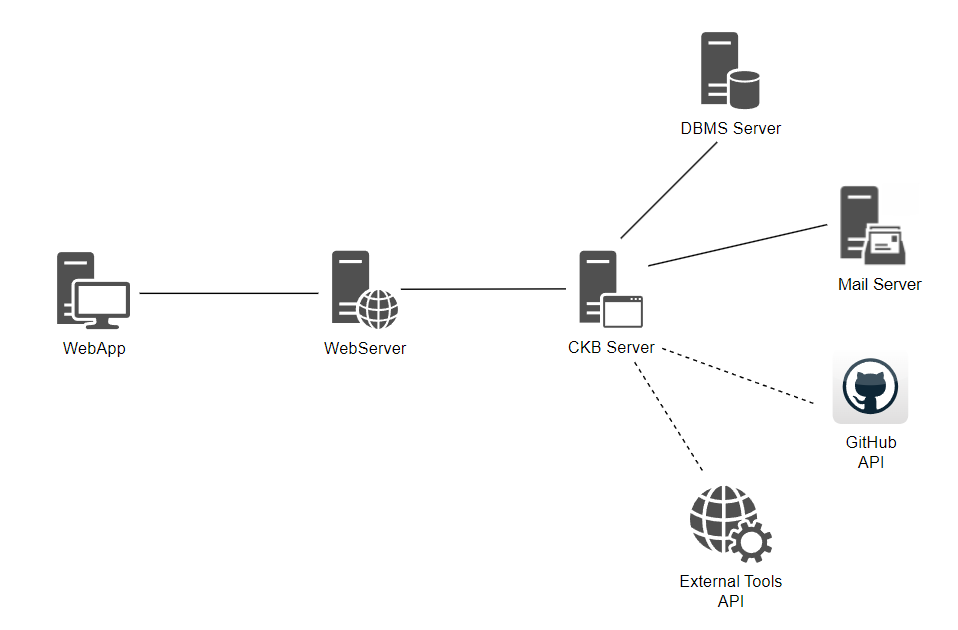
\includegraphics[width=1\linewidth]{CD_DD/Overview.png}
        \caption{S\&C Overview.}
        \label{fig:CKB_overview}%
    \end{center}
\end{figure}

\noindent Client side:
\begin{itemize}
    \item WebApp: Represents the User Interface of the system, providing access through a web application to the offered services such as registration, login, updating profile overview, creating internships, searching and applying for internships, creating tasks for candidates, submitting complaints or providing feedback. It’s responsible for all the User interactions, and it communicates with the main server through the Web Server, using secure protocols like HTTPS.
\end{itemize}
\noindent Server side:
\begin{itemize}
    \item \textbf{Web Server:} handles communication with Users, receiving and processing their inputs. Additionally, it provides load balancing for requests, distributing them among various replicas of the S\&C Server. It also manages the User sessions.
    \item \textbf{S\&C Server:} the core of the system, contains most of the logic of the software and handles interactions between different components. It also coordinates the communication with the DBMS, triggers the recommendation algorithm through the External Tools API and sends notifications to the users. It serves as the primary server for the entire website and is replicated across multiple machines to handle a high volume of requests.
    \item \textbf{DBMS Server:} stores data related to Users, Internships, Resumes, Complaints and Feedback. It acts as the repository for essential information.
    \item \textbf{Mail Server:} is responsible for sending confirmation email when a new User registers on S\&C, enhancing the User registration process.
    \item \textbf{External Tools API:} used to run the recommendation algorithm. It also takes feedback in inputs to reinforce the algorithm over time, ensuring better accuracy in the matching process.
\end{itemize}

\section{Component View}
\label{sec:component_view}%

\subsection{High Level Diagram}
\label{subsec:high_level_diagram}%

\begin{figure}[H]
    \begin{center}
        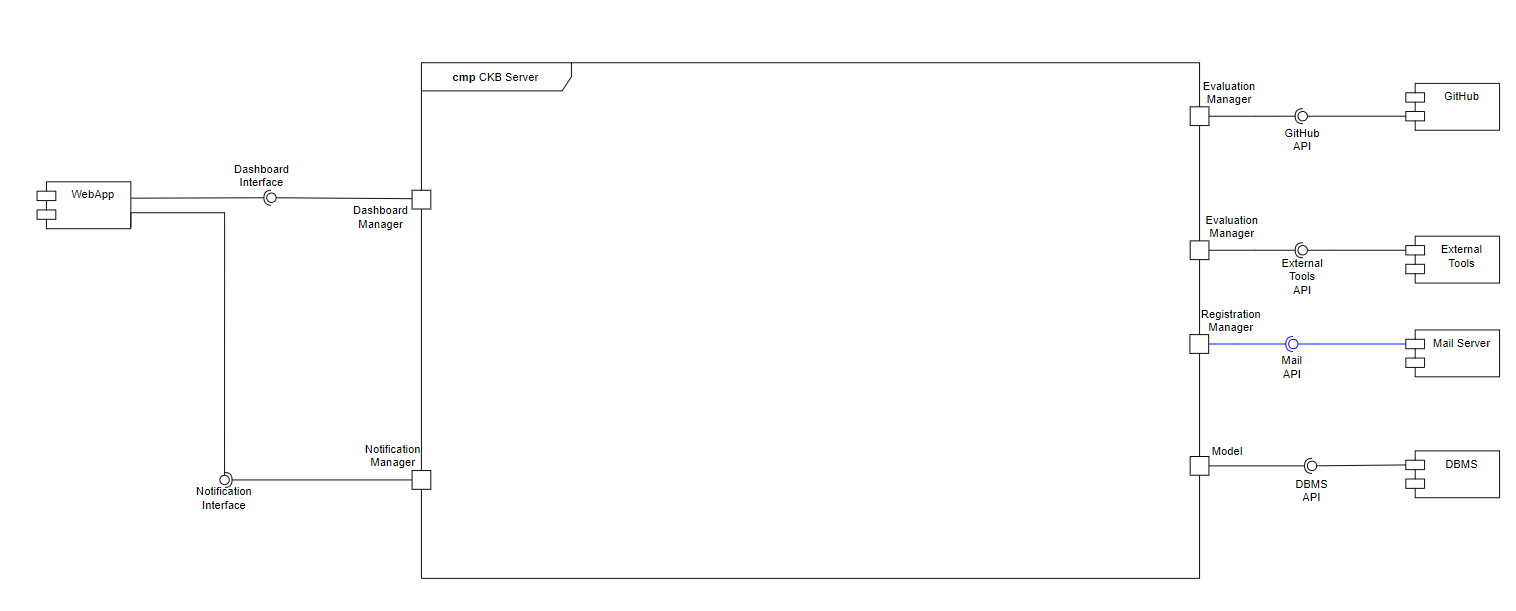
\includegraphics[width=1\linewidth]{CD_DD/HighLevel.png}
        \caption{High Level Diagram.}
        \label{fig:high_level_diagram}%
    \end{center}
\end{figure}

\noindent In the figure above is the high level component diagram of S\&C where it’s represented the external components of S\&C and how they communicate with the S\&C server, in particular:
\begin{itemize}
    \item \textbf{WebApp}: serves as the external access point for Users, allowing communication with the S\&C Server through the Dashboard Interface—the sole means for Client-Server interaction from the User side. The S\&C Server can relay notifications, such as Student uploading overviews or Internship creation, to Users through the Notification Interface.
    \item \textbf{DBMS:} is the storage repository for all User data, Internships, Feedback and Complaints. It communicates with the S\&C Server via the DBMS API, which is connected to the Model component.
    \item \textbf{Mail Server:} responsible for sending registration confirmation emails, the Mail Server communicates with the S\&C Server using the Mail API interface. This interface is linked to the Registration Manager component, which oversees the User registration process..
    \item \textbf{External Tools:} external application used for running and reinforcing a sophisticated recommendation algorithm. It communicates with the S\&C Server through the External Tools API, connecting to the Recommendation Manager component. The Recommendation Manager handles the notification process for the matching phase of the system.
\end{itemize}

\subsection{Low Level Diagram}
\label{subsec:low_level_diagram}%

\begin{figure}[H]
    \begin{center}
        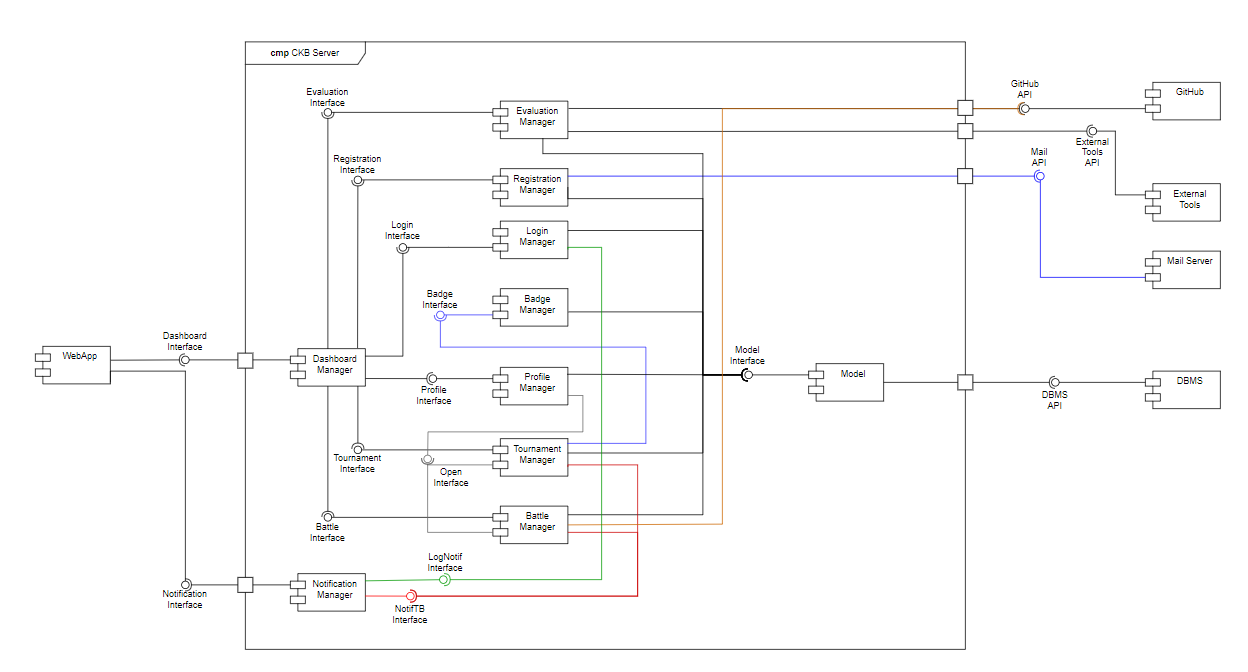
\includegraphics[width=1\linewidth]{CD_DD/LowLevel.png}
        \caption{Low Level Diagram.}
        \label{fig:low_level_diagram}%
    \end{center}
\end{figure}

\noindent The figure above represents the complete architecture of S\&C website with each components inside the S\&C Server:
\begin{itemize}
    \item \textbf{Dashboard Manager:} This fundamental component orchestrates all the communication between User and the S\&C website. Users communicate with the system through the Dashboard Interface, so the Dashboard Manager address all the requests to the right component, depending on the User's needs. 
    \item \textbf{Model:} This component represents the dataset of the server, and it act as a mask to the database server, so every component have to interface with it to access data from DBMS, which will access it directly through the DBMS API. 
    \item \textbf{Recommendation Manager:}  The component that handles everything about the recommendation phase of the system. It periodically triggers a new computation for finding new matches between students and internships, and it does that by using the External Tools API, which communicates directly with the system in which the computation take place. It also communicate with the model for retrieving all the information necessary to the user to visualize the correct recommendation list, each time there is a new request incoming from the Dashboard Manager. This component additionally communicates with the Profile Manager through the View Profile Interface, every time that a company, from it's recommendation list wants to check the profile overview of a Student.
    \item \textbf{Registration Manager:} This components handles the registration of new Users on the system. The User when trying to create a new account interacts with the Dashboard Manager, which contacts the Registration Manager through the Registration interface. Then the Registration Manager handle the request and manages to contact the Mail Server through the Mail API, to send a confirmation email to the new User. Once this is done it uses the Model through the Model Interface for saving user's information on the DBMS.
    \item \textbf{Login Manager:} This component handle the Login process for registered Users. When a User attempts to Login, the Dashboard Manager address the request to this component, which contacts the Model through the Model Interface to retrieve data from the DBMS and so authenticate the User. 
    \item \textbf{Profile Manager:} Component that allows Students to create their profile overview. When a Student starts the process to complete it's profile, the Dashboard Manager forwards the requests to the Profile manager using the Profile Interface. The Profile Manager communicates with the Model component through the Model Interface to store new information in the DBMS. It also manage to retrieve Students information when a company wants to view the overview of a Student within the recommendation list.
    \item \textbf{Internship Manager:} This component allow the Companies to create, modify and visualize internships. When a company wants to publish a new internship, interacts with the dashboard manager, which forwards the requests to the Internship Manager. This component manage to save new published internship, modify the status or retrieve information for internship search from the Model component, interacting with it via the Model Interface.
    \item \textbf{Interview Manager:} This is the main component of the interview phase of an internship. When a company wants to start preparing tasks or submit them to candidates, interacts with the Dashboard Manager, who forwards the requests to the Interview Manager, who manage to interact with the Model through the Model Interface for saving information. It can also notify the candidates when the tasks are ready to be carried out, or results are ready, contacting the Notification Manager module through the InterviewNotif Interface.
    \item \textbf{Complaints Manager:} This component handles the complaints related to an internship. When a User wants to file a complaint about an internship, interact with the Dashboard Manager, who forwards the requests to the Complaint Manager through the Complaint Interface, which needs to Notify the University of the Student related complaint, contacting the Notification Manager module through the InterviewNotif Interface. It can also store the complaints on the model for the purpose of reinforcing the algorithm.
    \item \textbf{Feedback Manager:} This component has the tasks of handling the feedback process. When a User wants to provide a feedback about an internship, it interacts with the Dashboard Manager, who forwards the requests to the Feedback Manager, that manage to save the new data on the DBMS contacting the Model through the Model Interface. By doing that, it allows the Recommendation Manager to retreive useful information from the DBMS to reinforce the Recommendation algorithm.
    \item \textbf{Notification Manager:} Component that handles each notification that has to be sent to the Users, in particular when a new match has been found from the recommendation algorithm, it sends a notification both to the Student and the Company related with that match; when the interview phase is completed, it sends the notification to all the candidates informing them wether they've been selected or not; when a new complaint is made from a company or a student, it notify the university that has to handle it. All the communication from other components to this are made through the InterviewNotif Interface, ComplNotif Interface or the Recommendation Interface, and it communicates with the web app through the Notification Interface..
\end{itemize}

\subsection{Evaluation Manager}
\label{subsec:evaluation_manager}%

\begin{figure}[H]
    \begin{center}
        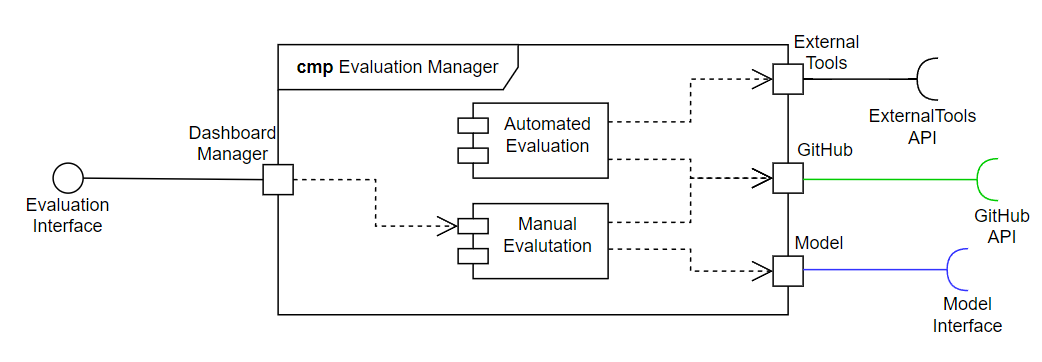
\includegraphics[width=1\linewidth]{CD_DD/Evaluation Manager.png}
        \caption{Evaluation Manager.}
        \label{fig:evaluation_manager}%
    \end{center}
\end{figure}

\noindent The Evaluation Manager is composed by two other sub-components that handles the two different evaluation method of a STG code:

\begin{itemize}
    \item \textbf{Automated Evaluation component:} utilized by the CKB system to automatically evaluate STG code whenever a new push is made to the STG's forked repository on GitHub. When a code update occurs, GitHub communicates with the Automated Evaluation component through the GitHub API. Subsequently, the Automated Evaluation component sends the code to External Tools via the External Tools API, where the code undergoes testing and evaluation. Upon receiving the evaluation results, the Automated Evaluation component, through the Model interface, communicates with the Model component. The Model component utilizes the DBMS API to update the new score in the relevant DBMS section associated with the corresponding Battle.
    \item \textbf{Manual Evaluation component:} comes into play when an ED wishes to manually assess an STG code. The process begins with the WebApp, which, through the Dashboard Interface, requests the STG code from the Dashboard Manager. The Dashboard Manager then communicates this request to the Manual Evaluation component through the Evaluation Interface. Subsequently, the Manual Evaluation component communicates with the GitHub API to retrieve the source code from the STG's forked repository, allowing the ED to analyze it. Once the evaluation is complete and the ED decides to update the score, the Manual Evaluation component, through the Model Interface, communicates with the Model component. The Model component, utilizing the DBMS API, updates the score in the DBMS, ensuring the manual evaluation results are recorded appropriately.
\end{itemize}

\subsection{Badge Manager}
\label{subsec:badge_manager}%

\begin{figure}[H]
    \begin{center}
        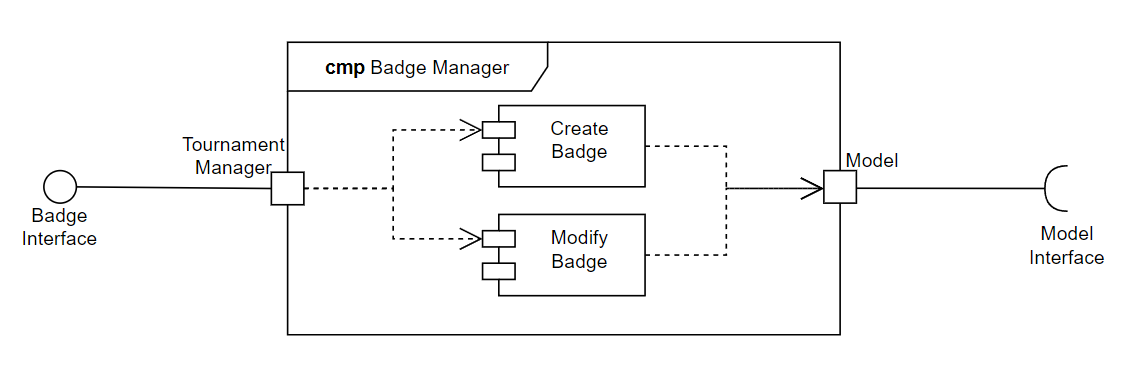
\includegraphics[width=1\linewidth]{CD_DD/Badge Manager.png}
        \caption{Badge Manager.}
        \label{fig:badge_manager}%
    \end{center}
\end{figure}

\noindent The Badge Manager is the component used by the CKB system to handle the creation and the modification of the Badges during the Tournament creation:

\begin{itemize}
    \item \textbf{Create Badge component:} activated when an ED intends to create a new Badge for a newly created Tournament. The initiation of this process is through the Create Tournament component, a sub-component of the Tournament Manager. The Create Tournament component, via the Badge Interface, sends a request to the Create Badge component, allowing the ED to define the Badge with its specific settings and parameters, such as the criteria STs must fulfill to obtain it. Following the Badge creation, the Create Badge component, through the Model Interface, communicates with the Model component, ensuring the newly created Badge is added to the DBMS.
    \item \textbf{Modify Badge component:} engaged when an ED aims to modify an existing Badge that was previously created for another Tournament. The process is initiated by the Create Tournament component, a sub-component of the Tournament Manager. The Create Tournament component, via the Badge Interface, sends a request to the Modify Badge component, allowing the ED to adjust parameters associated with an existing Badge, specifying new criteria for STs to fulfill. Once the Badge is successfully modified, the Modify Badge component, through the Model Interface, communicates with the Model component. This communication ensures that the updated Badge information is reflected in the DBMS.
\end{itemize}

\subsection{Profile Manager}
\label{subsec:profile_manager}%

\begin{figure}[H]
    \begin{center}
        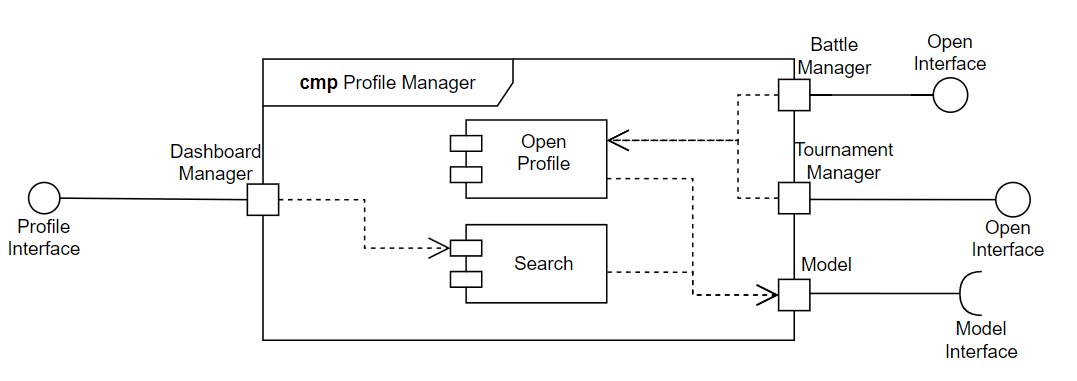
\includegraphics[width=1\linewidth]{CD_DD/Profile Manager.png}
        \caption{Profile Manager.}
        \label{fig:profile_manager}%
    \end{center}
\end{figure}

\noindent The Profile Manager is the component used by the CKB system to handle the research of a User’s profile and the visualization of another User’s profile when the User clicks on a nickname within the Tournament or Battle dashboard:

\begin{itemize}
    \item \textbf{Search component:} responsible for managing the profile search process when a User enters a nickname or keyword into the search bar across various CKB pages. When a User initiates a search by entering another User's nickname or a relevant keyword, the Dashboard Manager communicates with the Search component through the Profile Interface. The Search component then forwards the search request to the Model component via the Model Interface. Subsequently, the Model component retrieves the profile information from the DBMS. The retrieved information is then presented to the User, allowing him to visualize the searched User's profile.
    \item \textbf{Open Profile component:} manages the retrieval of a User's profile when a User clicks on a nickname within a Tournament or Battle dashboard. When a User clicks on another User's nickname in a Tournament or Battle dashboard, the Dashboard Manager communicates with the View component within the Tournament or Battle Manager. The View component forwards the request to the Open Profile component through the Open Interface. The Open Profile component communicates with the Model component via the Model Interface. This communication with the Model component facilitates the retrieval of the User's profile information from the DBMS. The retrieved profile information is then presented to the User, allowing them to view the selected User's profile.
\end{itemize}

\subsection{Tournament Manager}
\label{subsec:tournament_manager}%

\begin{figure}[H]
    \begin{center}
        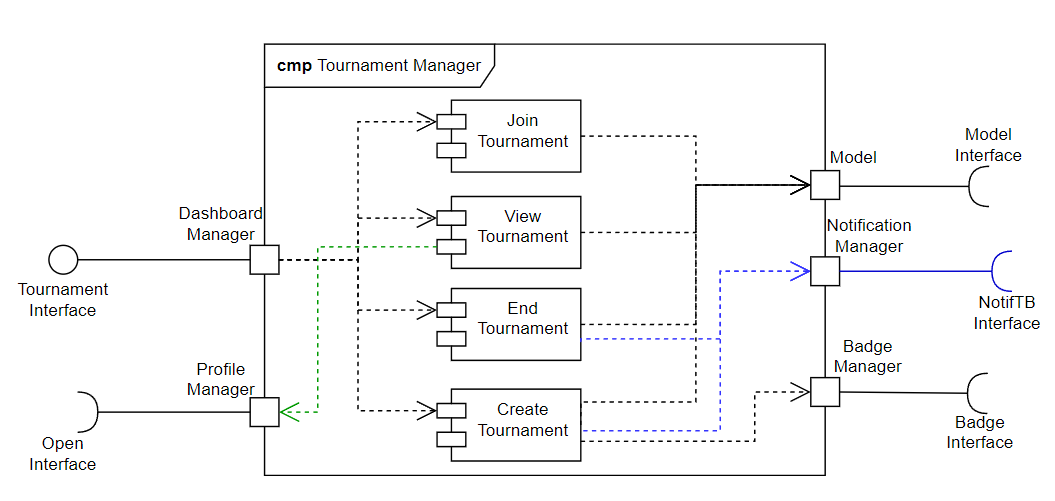
\includegraphics[width=1\linewidth]{CD_DD/Tournament Manager.png}
        \caption{Tournament Manager.}
        \label{fig:tournament_manager}%
    \end{center}
\end{figure}

\noindent The Tournament Manager is the component used by the CKB system to handle every aspect of the Tournament, from the creation to the end going through the Join and the View sub-components:

\begin{itemize}
    \item \textbf{Create Tournament component:} utilized when an ED initiates the creation of a new Tournament. The ED communicates with the Dashboard Manager through the Dashboard Interface, which then directs the request to the Create Tournament component. This component sends back a creation form for the ED to fill. Once completed, the Create Tournament component communicates the data to the Model component through the Model Interface, adding the information to the DBMS via the DBMS API. If the ED grants permissions to other EDs, the Create Tournament component communicates with the Notification Manager through the NotifTB Interface to notify the specified EDs. Additionally, notifications are sent to all the STs via the Notification Manager, informing them of the new Tournament. Throughout the Tournament creation process, the Create Tournament component also communicates with the Badge Manager through the Badge Interface, allowing the ED to create or modify Badges associated with the Tournament.
    \item \textbf{Join Tournament component:} activated when an ST wishes to join a Tournament. The ST communicates with the Dashboard Manager through the Dashboard Interface, and the request is forwarded to the Join Tournament component. This component communicates through the Model Interface with the Model component to add the ST to the Tournament participant list in the DBMS through the DBMS API. 
    \item \textbf{View Tournament component:} used by the CKB system to let the User visualize the Tournament page with all the information, like the available Battles and the Dashboard with the STs score. When a User wants to search a Tournament it writes the Tournament name or a keyword in the search bar and it communicates with the Dashboard Manager through the Dashboard Interface that forwards the request to the View Tournament component that communicates with the Model component through the Model Interface to retrieve all the information from the DBMS through the DBMS API and let the User visualize the Tournament page. The same communication is made when a User clicks on a Tournament name in another User’s profile or in his main dashboard page. This component also manages the open profile operation when a User wants to visualize another User’s profile from the Tournament dashboard; when a User clicks on another User’s nickname in the Tournament dashboard the Dashboard Manager communicates through the Dashboard Interface with the View Tournament component that forwards the request to the the Profile Manager through the Open Interface.
    \item \textbf{End Tournament component:} triggered when an ED decides to close a Tournament, preventing further ST participation and ED creation of Battles within it. The ED communicates with the Dashboard Manager through the Dashboard Interface, which forwards the request to the Close Tournament component. The Close Tournament component communicates with the Model component through the Model Interface, modifying the Tournament's status to make it non-joinable in the DBMS through the DBMS API. Additionally, the Close Tournament component communicates through the NotifTB Interface to the Notification Manager, which sends notifications to all STs who participated in the Tournament, informing them that final scores are ready for viewing.
\end{itemize}

\subsection{Battle Manager}
\label{subsec:battle_manager}%

\begin{figure}[H]
    \begin{center}
        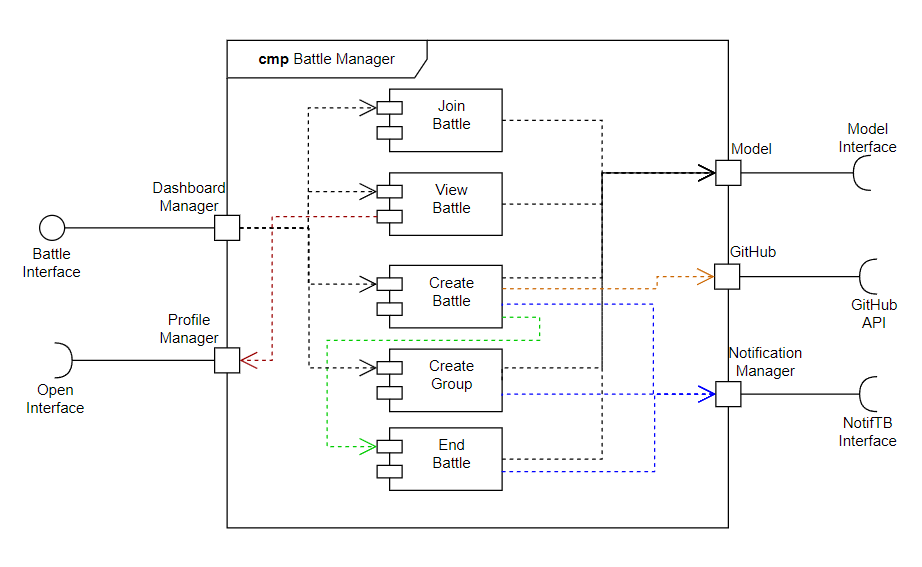
\includegraphics[width=1\linewidth]{CD_DD/Battle Manager.png}
        \caption{Battle Manager.}
        \label{fig:battle_manager}%
    \end{center}
\end{figure}

\noindent The Battle Manager is the component used by the CKB system to handle every aspect of the Battle, from the creation to the end going through the Join, the View and the Create Group sub-components:

\begin{itemize}
    \item \textbf{Create Battle component:} engaged when an ED wishes to create a new Battle within a Tournament. The ED communicates with the Dashboard Manager through the Dashboard Interface, forwarding the request to the Create Battle component. The Create Battle component responds by sending a creation form to be filled by the ED. Upon completion, the component communicates the data to the Model component through the Model Interface, adding the information to the DBMS through the DBMS API. Additionally, the Create Battle component communicates with the Notification Manager through the NotifTB Interface, notifying all STs who have joined the relevant Tournament about the new Battle. It also collaborates with the End Battle component to create a timer, ensuring that after the consolidation stage concludes, the End Tournament component notifies all STs about the availability of final grades. The Create Battle component also communicates with GitHub through the GitHub API to create a new repository and upload the code kata for the Battle. This repository is later forked by all STGs to submit their code.
    \item \textbf{Join Battle component:} activated when an ST intends to join a Battle. The ST communicates with the Dashboard Manager through the Dashboard Interface, and the request is forwarded to the Join Battle component. The Join Battle component, through the Model Interface, communicates with the Model component, adding the ST to the participant list of the Battle in the DBMS through the DBMS API.
    \item \textbf{View Battle component:} used by the CKB system to let the User visualize the Battle page with the dashboard including all the STGs score. When a User wants to visualize the Battle page it communicates with the Dashboard Manager through the Dashboard Interface that forwards the request to the View Battle component that communicates with the Model component through the Model Interface to retrieve all the information from the DBMS through the DBMS API and finally let the User visualize the Battle page. This component also manages the open profile operation when a User wants to visualize another User’s profile from the Battle dashboard; when a User clicks on another User’s nickname in the Battle dashboard the Dashboard Manager communicates through the Dashboard Interface with the View Tournament component that forwards the request to the the Profile Manager through the Open Interface.
    \item \textbf{Create Group component} engaged when STs want to create a new STG for a Battle. After joining a Battle before the registration deadline expires, an ST can create an STG to participate in the battle. The ST communicates with the Dashboard Manager through the Dashboard Interface, initiating a request to create a new STG. The request is forwarded to the Create Group component through the Battle Interface, allowing the ST to decide the STG name and invite other STs. Notifications are sent through the Notification Manager, which communicates with the Battle Manager through the NotifTB interface and with the WebApp through the Notification Interface. When the STG is confirmed, the Create Group component communicates through the Model Interface with the Model component to add the newly created STG to the DBMS through the DBMS API.
    \item \textbf{End Battle component:} activated to notify all STGs that the final scores of the Battle are available. When the consolidation stage concludes, and the timer created by the Create Battle component expires, the End Battle component communicates through the Model Interface with the Model component, updating the scores in the DBMS through the DBMS API. It also notifies all participating STs through the Notification Manager, communicating through the NotifTB Interface, that the final scores are accessible on the Battle page. Communication between the Notification Manager and the WebApp is facilitated through the Notification Interface.
\end{itemize}


\section{Deployment View}
\label{sec:deployment_view}%

In this section it will be shown the Deployment diagram of the CKB system, followed by a description of the components and their interactions:
\begin{figure}[H]
    \begin{center}
        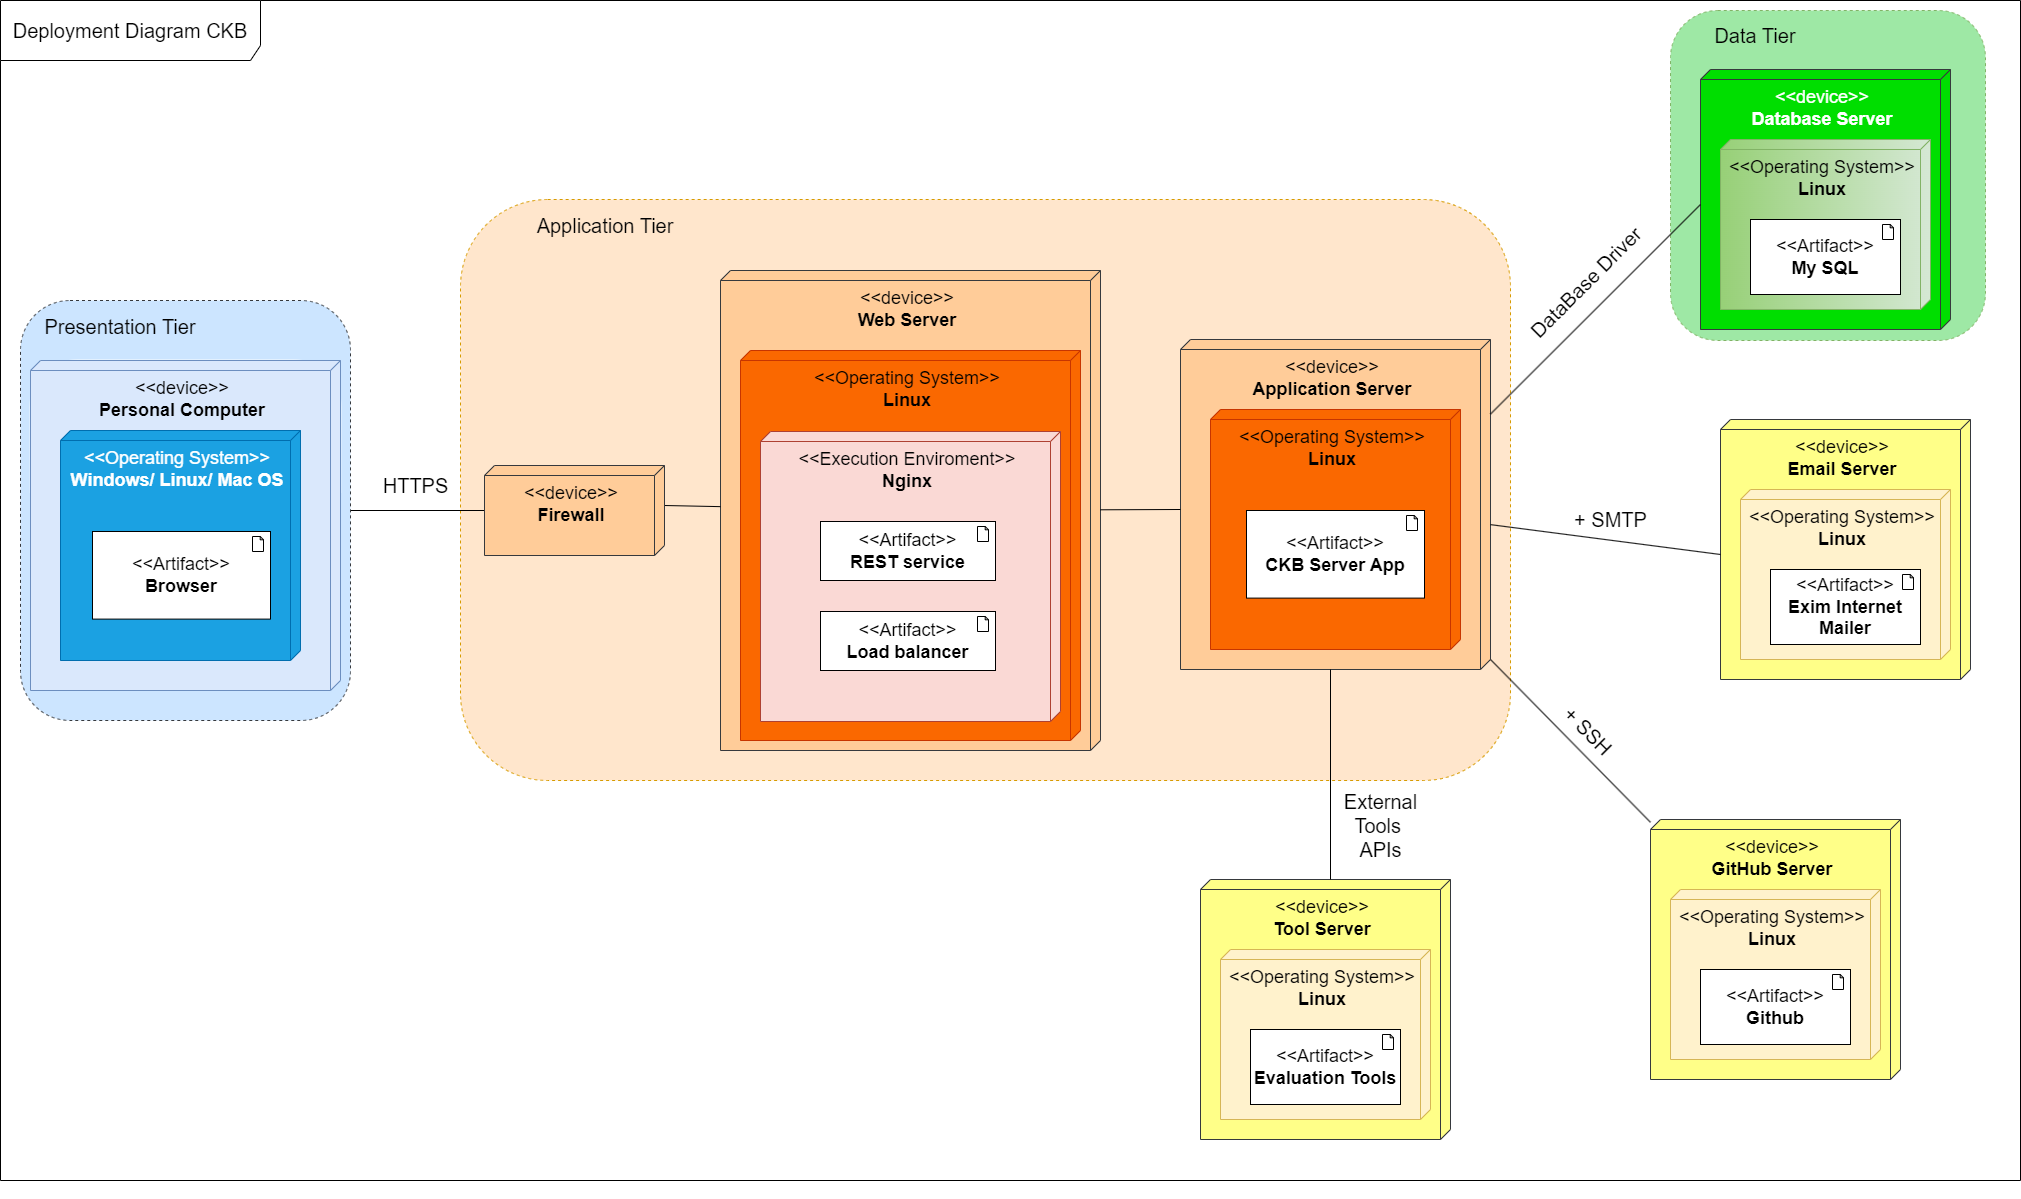
\includegraphics[width=1\linewidth]{CD_DD/DeploymentDiagram.png}
        \caption{Deployment Diagram.}
        \label{fig:Deployment_Diagram}%
    \end{center}
\end{figure}

\paragraph{Personal Computer:}
STs and EDs can access to the system by using any type of personal computer through their favorite web browser. The browser will communicate with the Web Server. Users can also use every device that allows them to search on a web browser, such as mobile phone, tablet, ecc.

\paragraph{Web Server:}
The Web Server provides access to the Application Server’s service to all the User that reaches the system through a web browser. In particular, the Web Server does not execute any business logic, but it simply does some load balancing on the receive requests from the client to the various Application Servers, in order to handle large User traffic.\\
It also provides to the client's browsers the HTML, JSON, Javascript and CSS files for making the rendering of the pages.

\paragraph{Firewall:}
It provides a way to limit the attack surface of any potential intruder by providing strict access rules.

\paragraph{Application Server:}
The application server contains the business logic of the entire system. Moreover, it communicates to the client through HTTPS protocol managed by the Web Server. The various requests coming from the Web Server are routed to the corresponding module thanks to the Dashboard Manager.\\
Furthermore, it communicates to the Database Server through the model gateway. This node is replicated in order to handle large user traffic.

\paragraph{Database Server:}
All the Data about Tournaments, Battles, Users, Groups and Badges are stored into the Database Server and managed by MySQL.\\
The various Application Servers can retrieve information on this node through the model module and the database driver.

\paragraph{Email Server:}
After the registration, Users have to click on the link sent by eMail to confirm their profile. The Application Server, immediately after the registration, contacts the Email Server through SMTP protocol to send the confirmation eMail to the User.

\paragraph{Github Server:}
The dialogs with the Application Server node occur during the different Battle phases: when the ED creates a new Battle also a GitHub repository is created containing the code kata of the Battle and it is subsequently forked from the various STG.\\
The GitHub Server is also periodically contacted for retrieving newly committed code on the main branch of the different STGs' repositories.
For those scopes, the Application Server shall communicate with the Github Server through the SSH protocol.


\paragraph{Tool Server:}
With the External Tool APIs the Application Server can contact the Tool Server and pass to it the code retrieved from the Github Server to be tested and evaluated.

\newpage
\section{Runtime View}
\label{sec:runtime_view}%

\subsection{SignUp as ED}
\begin{figure}[H]
    \begin{center}
        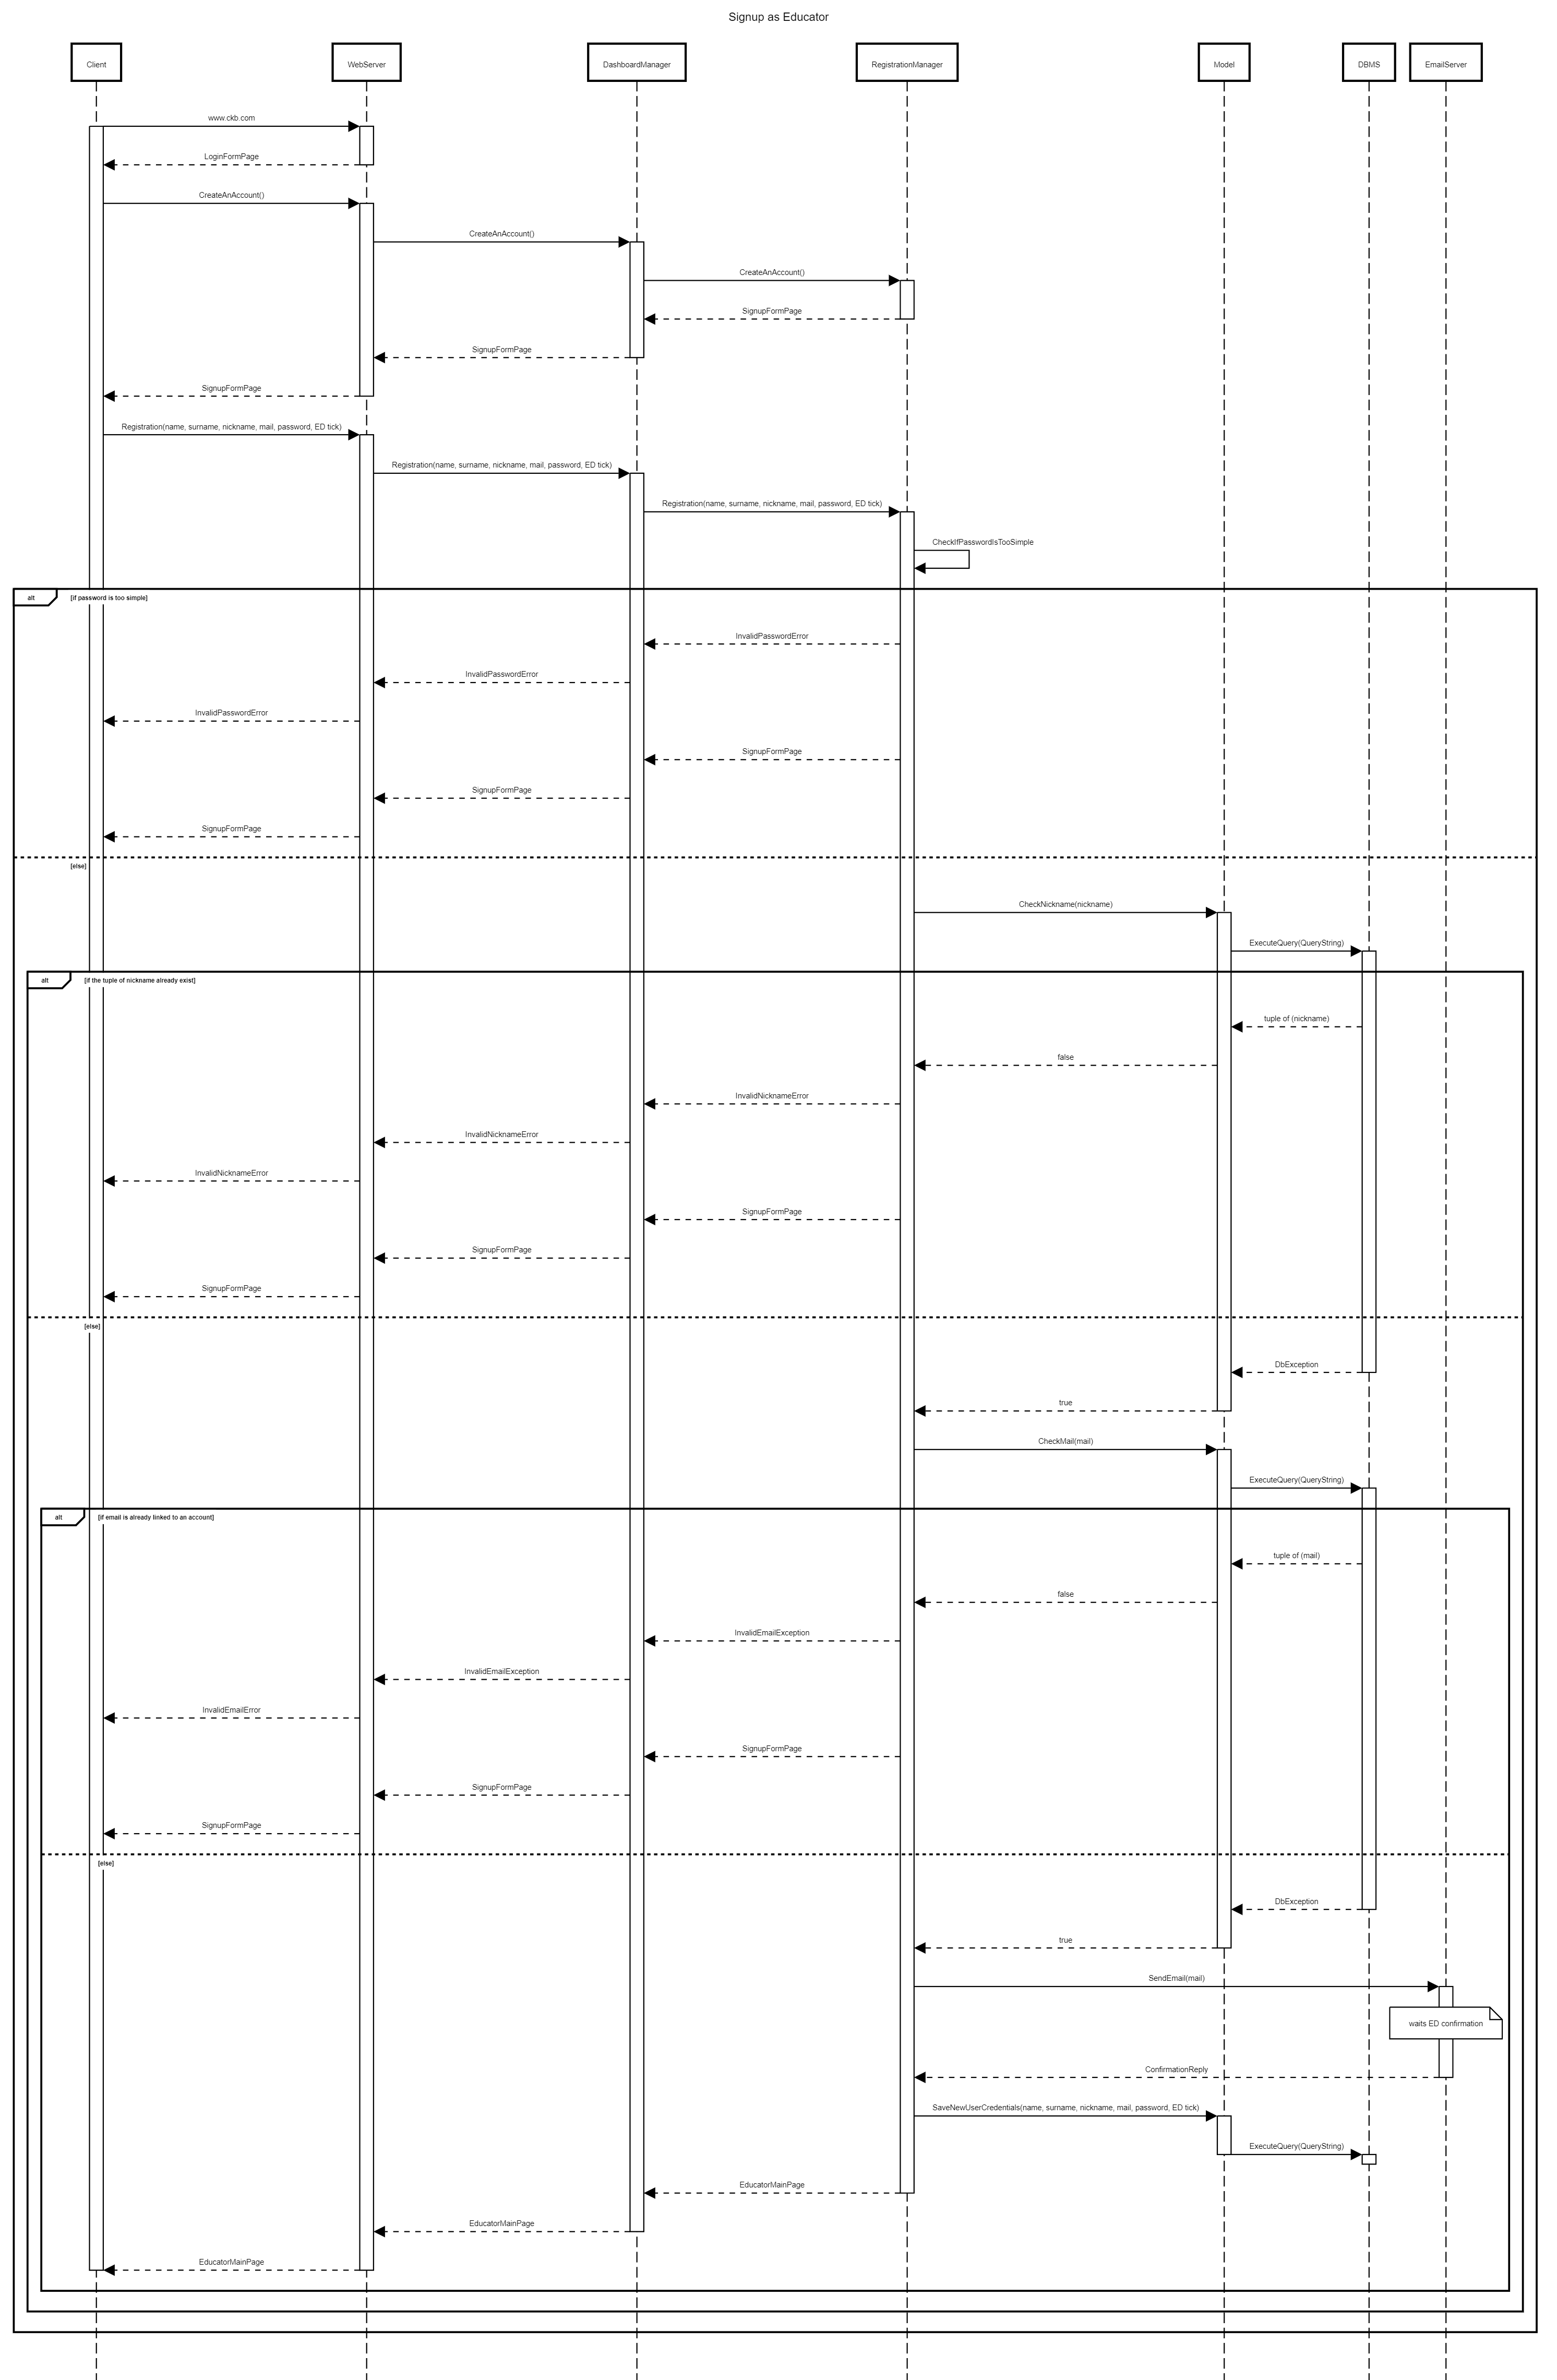
\includegraphics[width=0.8\linewidth]{RuntimeView/SignupED.png}
        \caption{Runtime view for 'SignUp as ED'.}
        \label{fig:runtime_signupasED}%
    \end{center}
\end{figure}

This sequence diagram represents the ED registration process.
The ED searches into the browser for the CKB Landing page and gets redirected to the “Login” page. After clicking on the "Create Account" button is redirected to the signup form. The ED fills out the form with his data, such as name, surname, nickname, mail and password and he ticks on the “Register as an Educator” option.
This form is forwarded to the DashboardManager that redirects the request to the RegistrationManager component. It does various checks on the sended parameters and, if everything is correct, sends an eMail to confirm  the registration. If the link in the mail is clicked the RegistrationManager saves the new profile into the Database (passing through the Model component that connects the Application Server with the DBMS) and shows to the ED the ED Homepage.


\subsection{SignUp as ST}
\begin{figure}[H]
    \begin{center}
        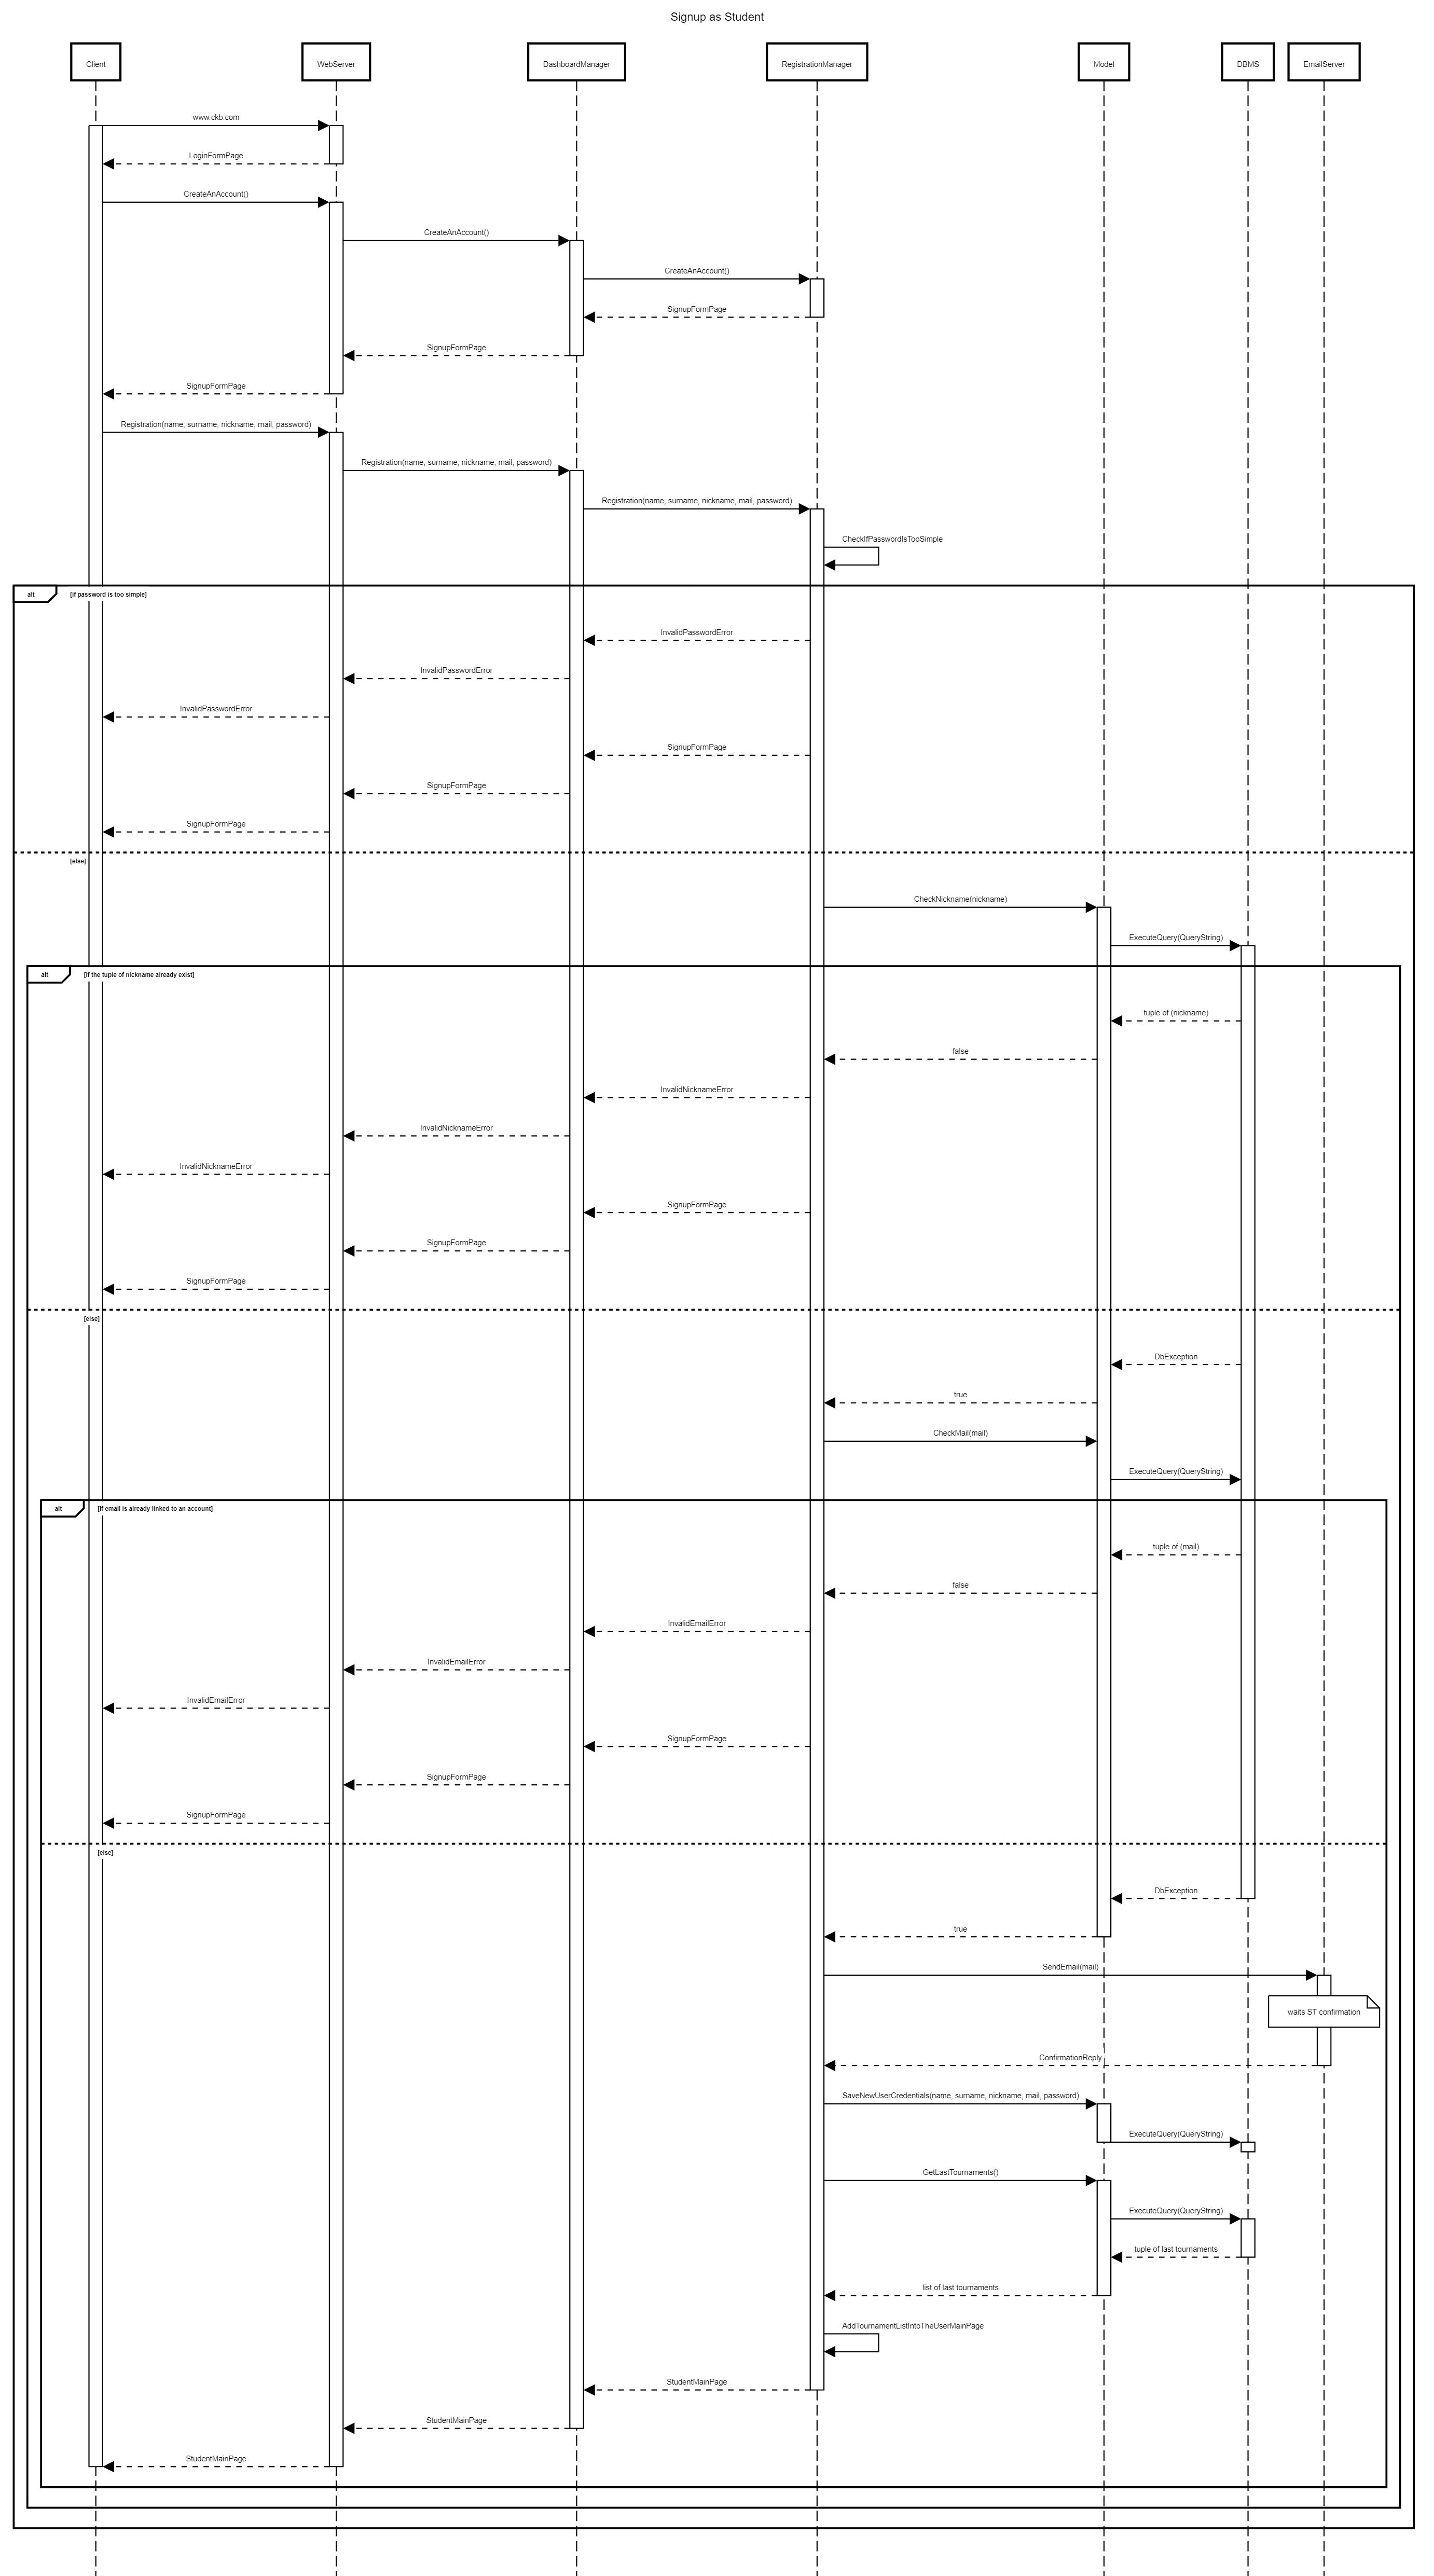
\includegraphics[width=0.8\linewidth]{RuntimeView/SignupAsST.png}
        \caption{Runtime view for 'SignUp as ST'.}
        \label{fig:runtime_signupasST}%
    \end{center}
\end{figure}

This sequence diagram represents the ST registration flow.
The ST searches into the browser for the CKB Landing page and gets the “Login” page.
After clicking on the "Create Account" button is redirected to the signup form.
The ST fills out the form with its data, such as name, surname, nickname, mail and password. 
This form is forwarded to the DashboardManager that redirects the request to the RegistrationManager component. It does various checks on the sended parameters and, if everything is correct, sends an eMail to confirm the registration.
If the link in the mail is clicked the RegistrationManager saves the new profile into the Database (passing through the Model component that connects the Application Server with the DBMS) and shows to the ST the ST Homepage.

\subsection{Login}
\begin{figure}[H]
    \begin{center}
        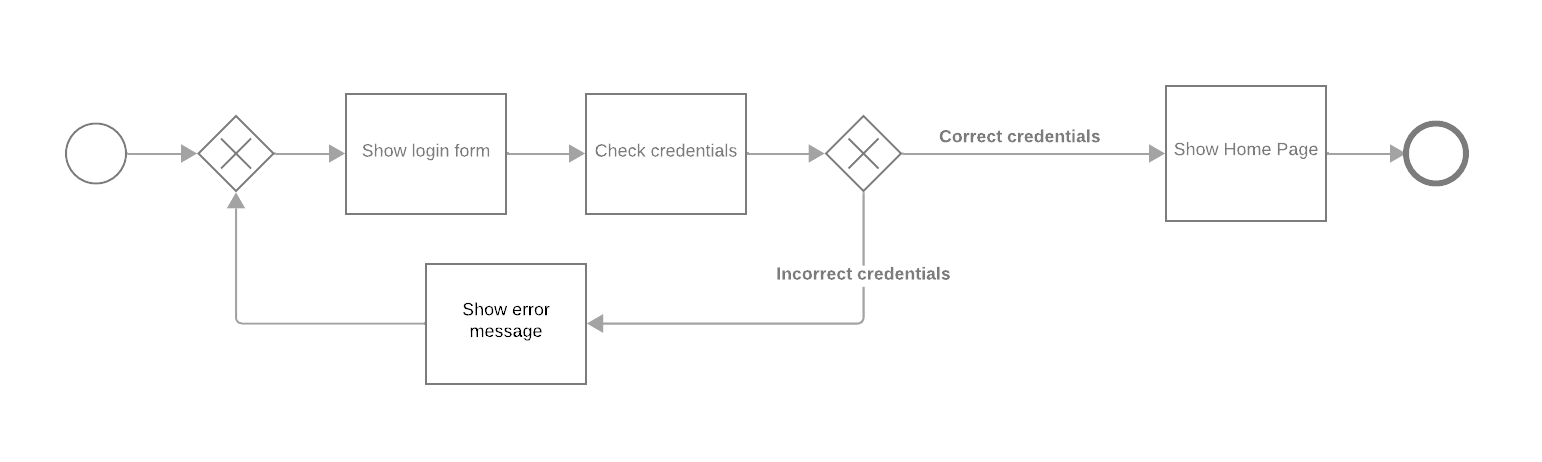
\includegraphics[height=0.8\pdfpageheight, width=0.8\linewidth]{RuntimeView/Login.png}
        \caption{Runtime view for 'Login'.}
        \label{fig:runtime_login}%
    \end{center}
\end{figure}
In this sequence diagram is explained how the login operation works.
The User searches into the browser for the CKB Landing page and gets the login page.
The User fills out the form with his credentials (nickname and password) and he sends it to the DashboardManager that redirects the request to the LoginManager that checks the credentials through the Model component.
The Model retrieves the User information from the DBMS and indicates to the LoginManager if the user is an ED or a ST.
The LoginManager adds the User credentials into the User session and retrieves the notifications that the User has missed and shows them to him.
After that the LoginManager gets from DBMS the information for creating the two types of User main page and sends them to the User.


\subsection{Create a Tournament}
\begin{figure}[H]
    \begin{center}
        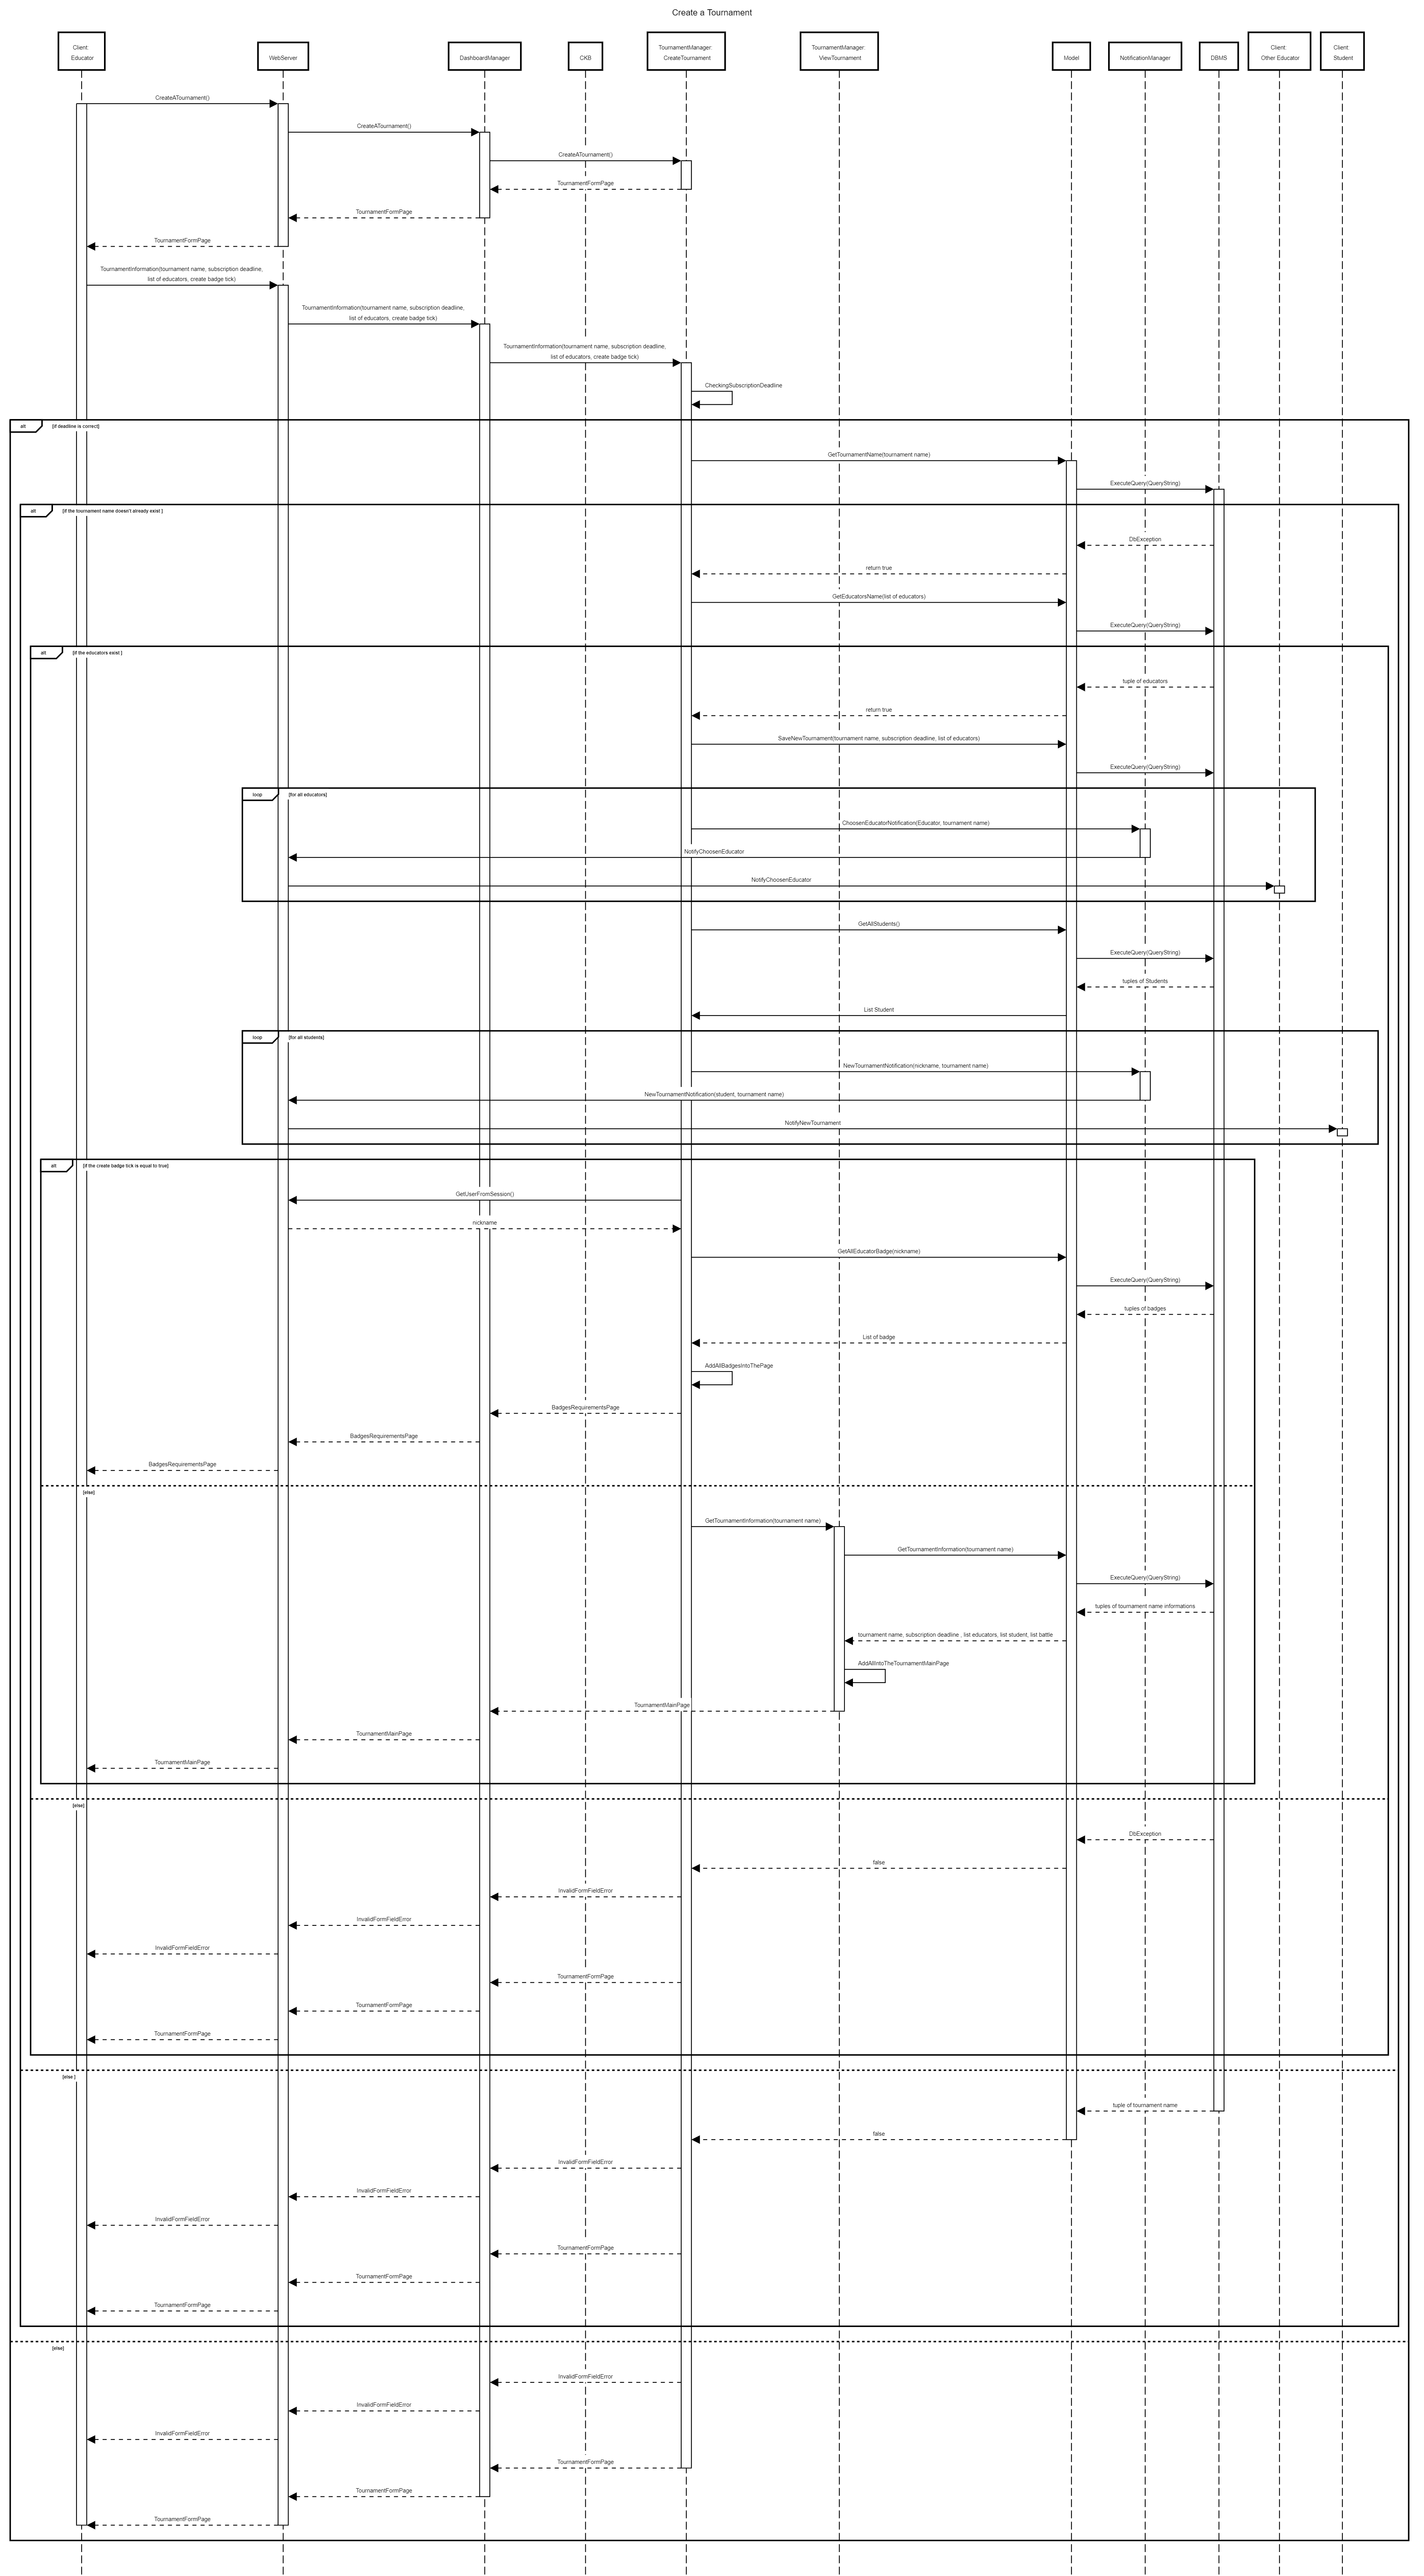
\includegraphics[width=0.8\linewidth]{RuntimeView/CreateTournament.png}
        \caption{Runtime view for 'Create a Tournament'.}
        \label{fig:runtime_createtournament}%
    \end{center}
\end{figure}
This sequence diagram represents the flow behind the create Tournament process.
The ED clicks on the “Create a new Tournament” button into the “ED Homepage” for retrieving the create Tournament form from the CreateTournament module. The ED fills out the form with the new Tournament information (Tournament name, subscription deadline, list of EDs) and if he wants to create or modify some Badges he ticks the “Create Badges for this Tournament” option. The form is sent to the DashboardManager that redirects the request to the CreateTournament module that, if the all parameters are corrects, saves the new Tournament into the DBMS and sends a notifications through the NotificationManager to all the invited EDs and to all the STs.
If the “Create Badges for this Tournament” option is ticked, the  CreateTournament module retrieves the ED’s Badges and redirects the ED to the “Create Badge” Page, if not the CreateTournament module calls the ViewTournament module in order to show the “ED Tournament” Page.


\subsection{Join a Tournament}
\begin{figure}[H]
    \begin{center}
        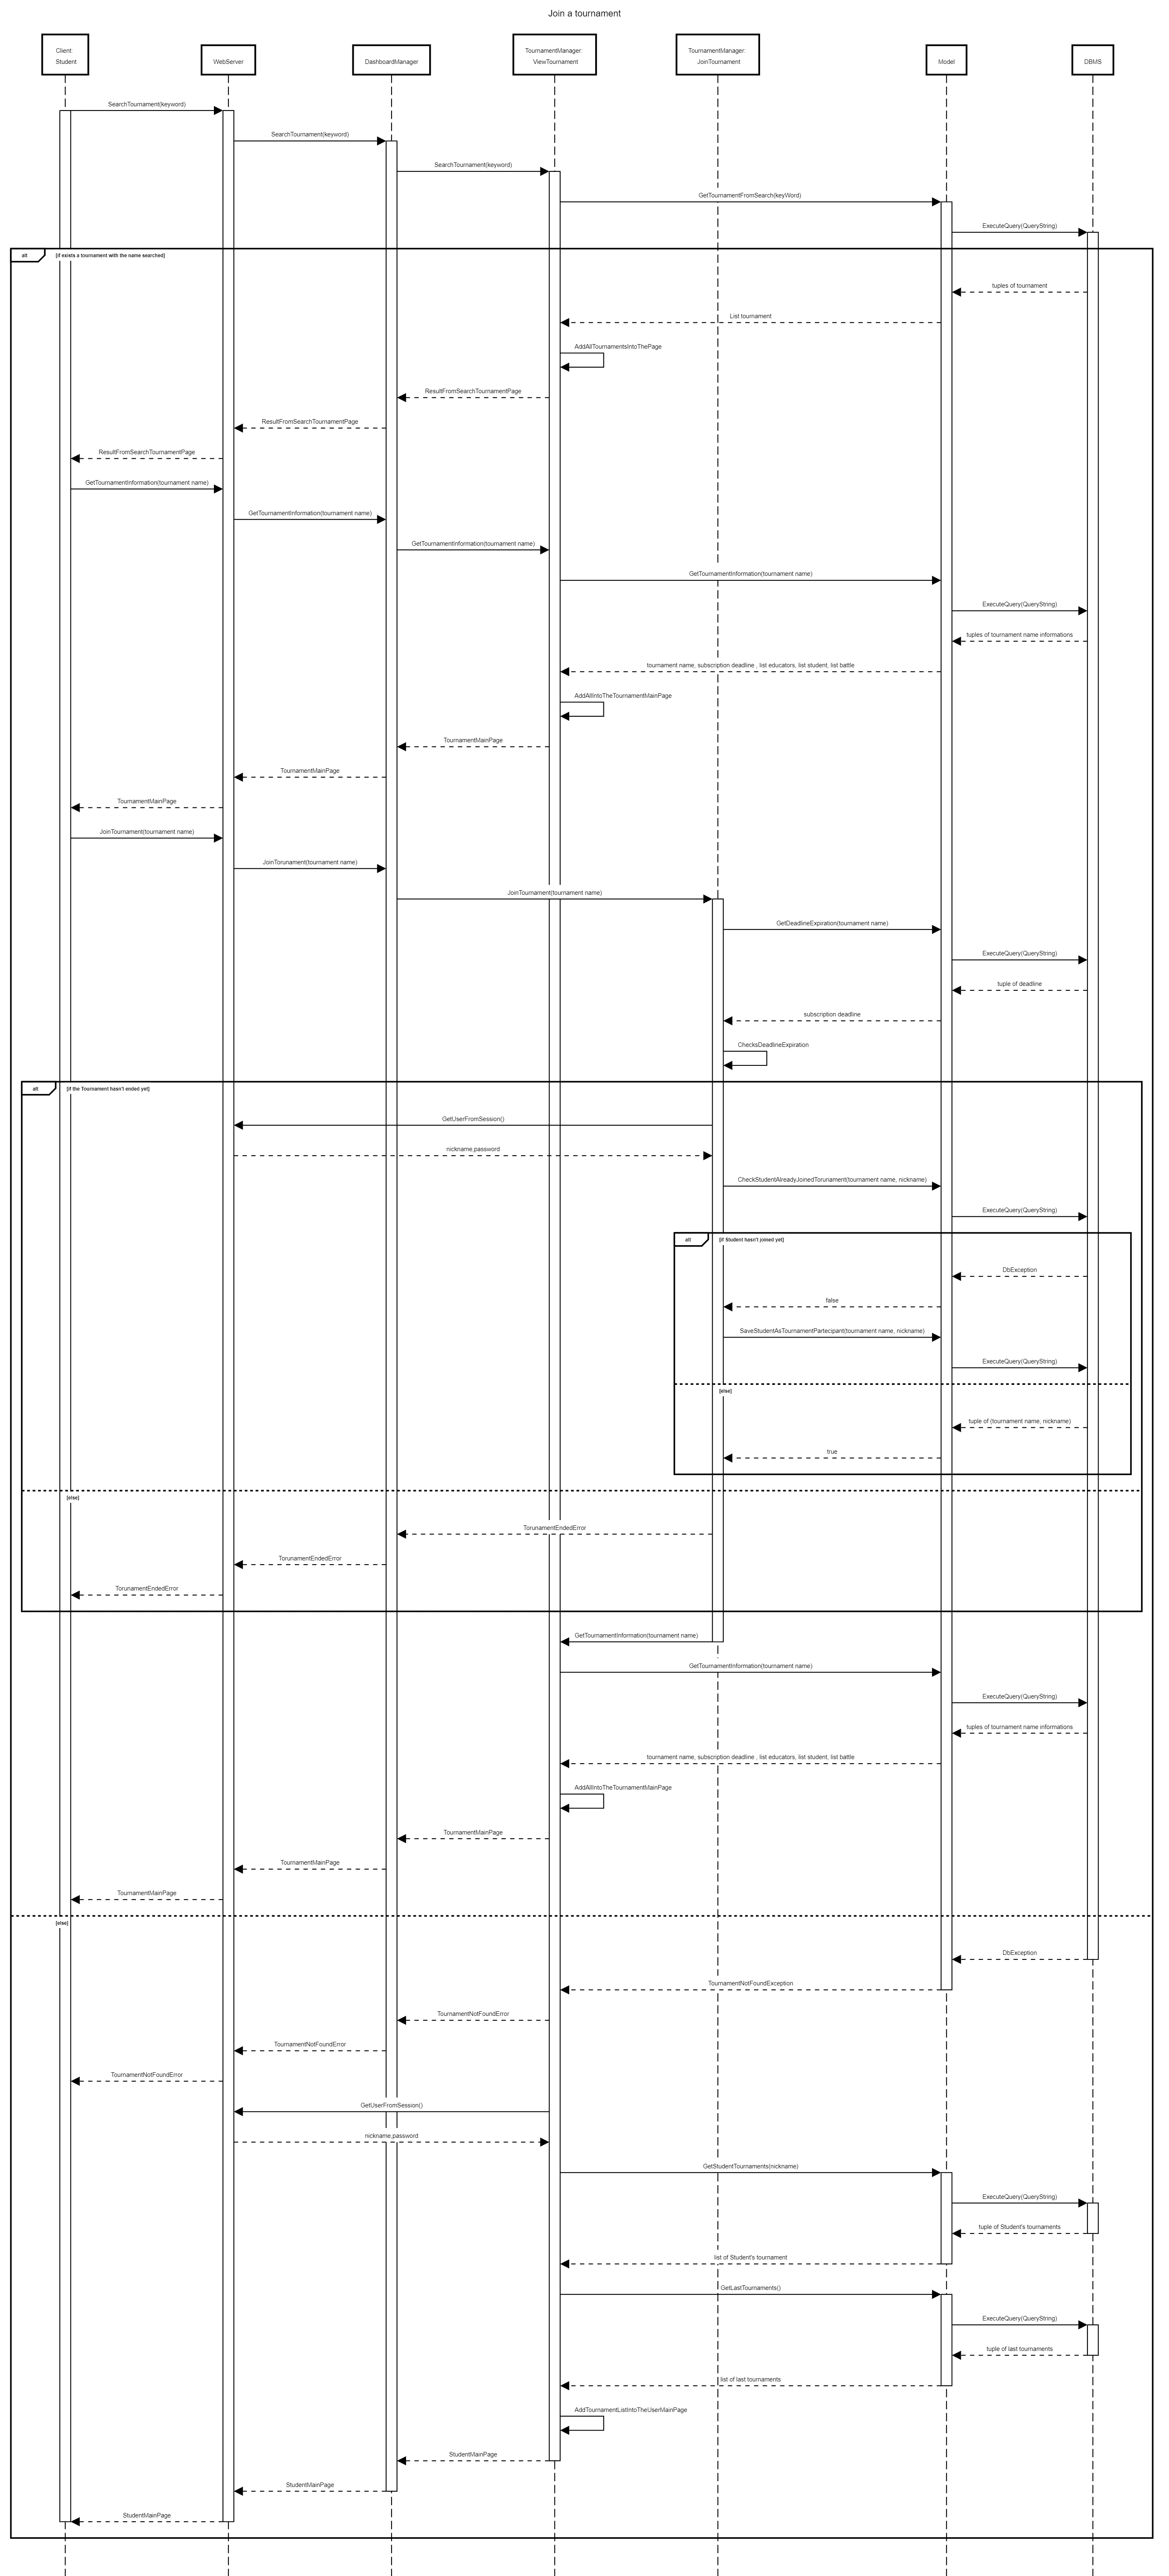
\includegraphics[height=0.8\pdfpageheight]{RuntimeView/JoinTournament.png}
        \caption{Runtime view for 'Join a Tournament'.}
        \label{fig:runtime_jointournament}%
    \end{center}
\end{figure}
This sequence diagram represents the flow behind the ‘Join Tournament’ operation for a ST.
The ST types a keyword into the search bar and sends it to the DashBoardManager that redirects the request to the ViewTournament module.
The ViewTournament module retrieves from the DBMS the list of Tournaments that corresponds to the searched keyword and, if it is not empty, shows it to the ST. The ST clicks on a Tournament and the ViewTournament module retrieves the information of that tournament from DBMS and shows them to the ST. The ST clicks on the “Join Tournament” button and his request is sent to the JoinTournament module that does some checks on the ST and in the Tournament. If all checks are passed the ST is saved into the DBMS as a Tournament participant and the “ST Tournament” page is shown to him through the ViewTournament module.


\subsection{Create a Battle}
\begin{figure}[H]
    \begin{center}
        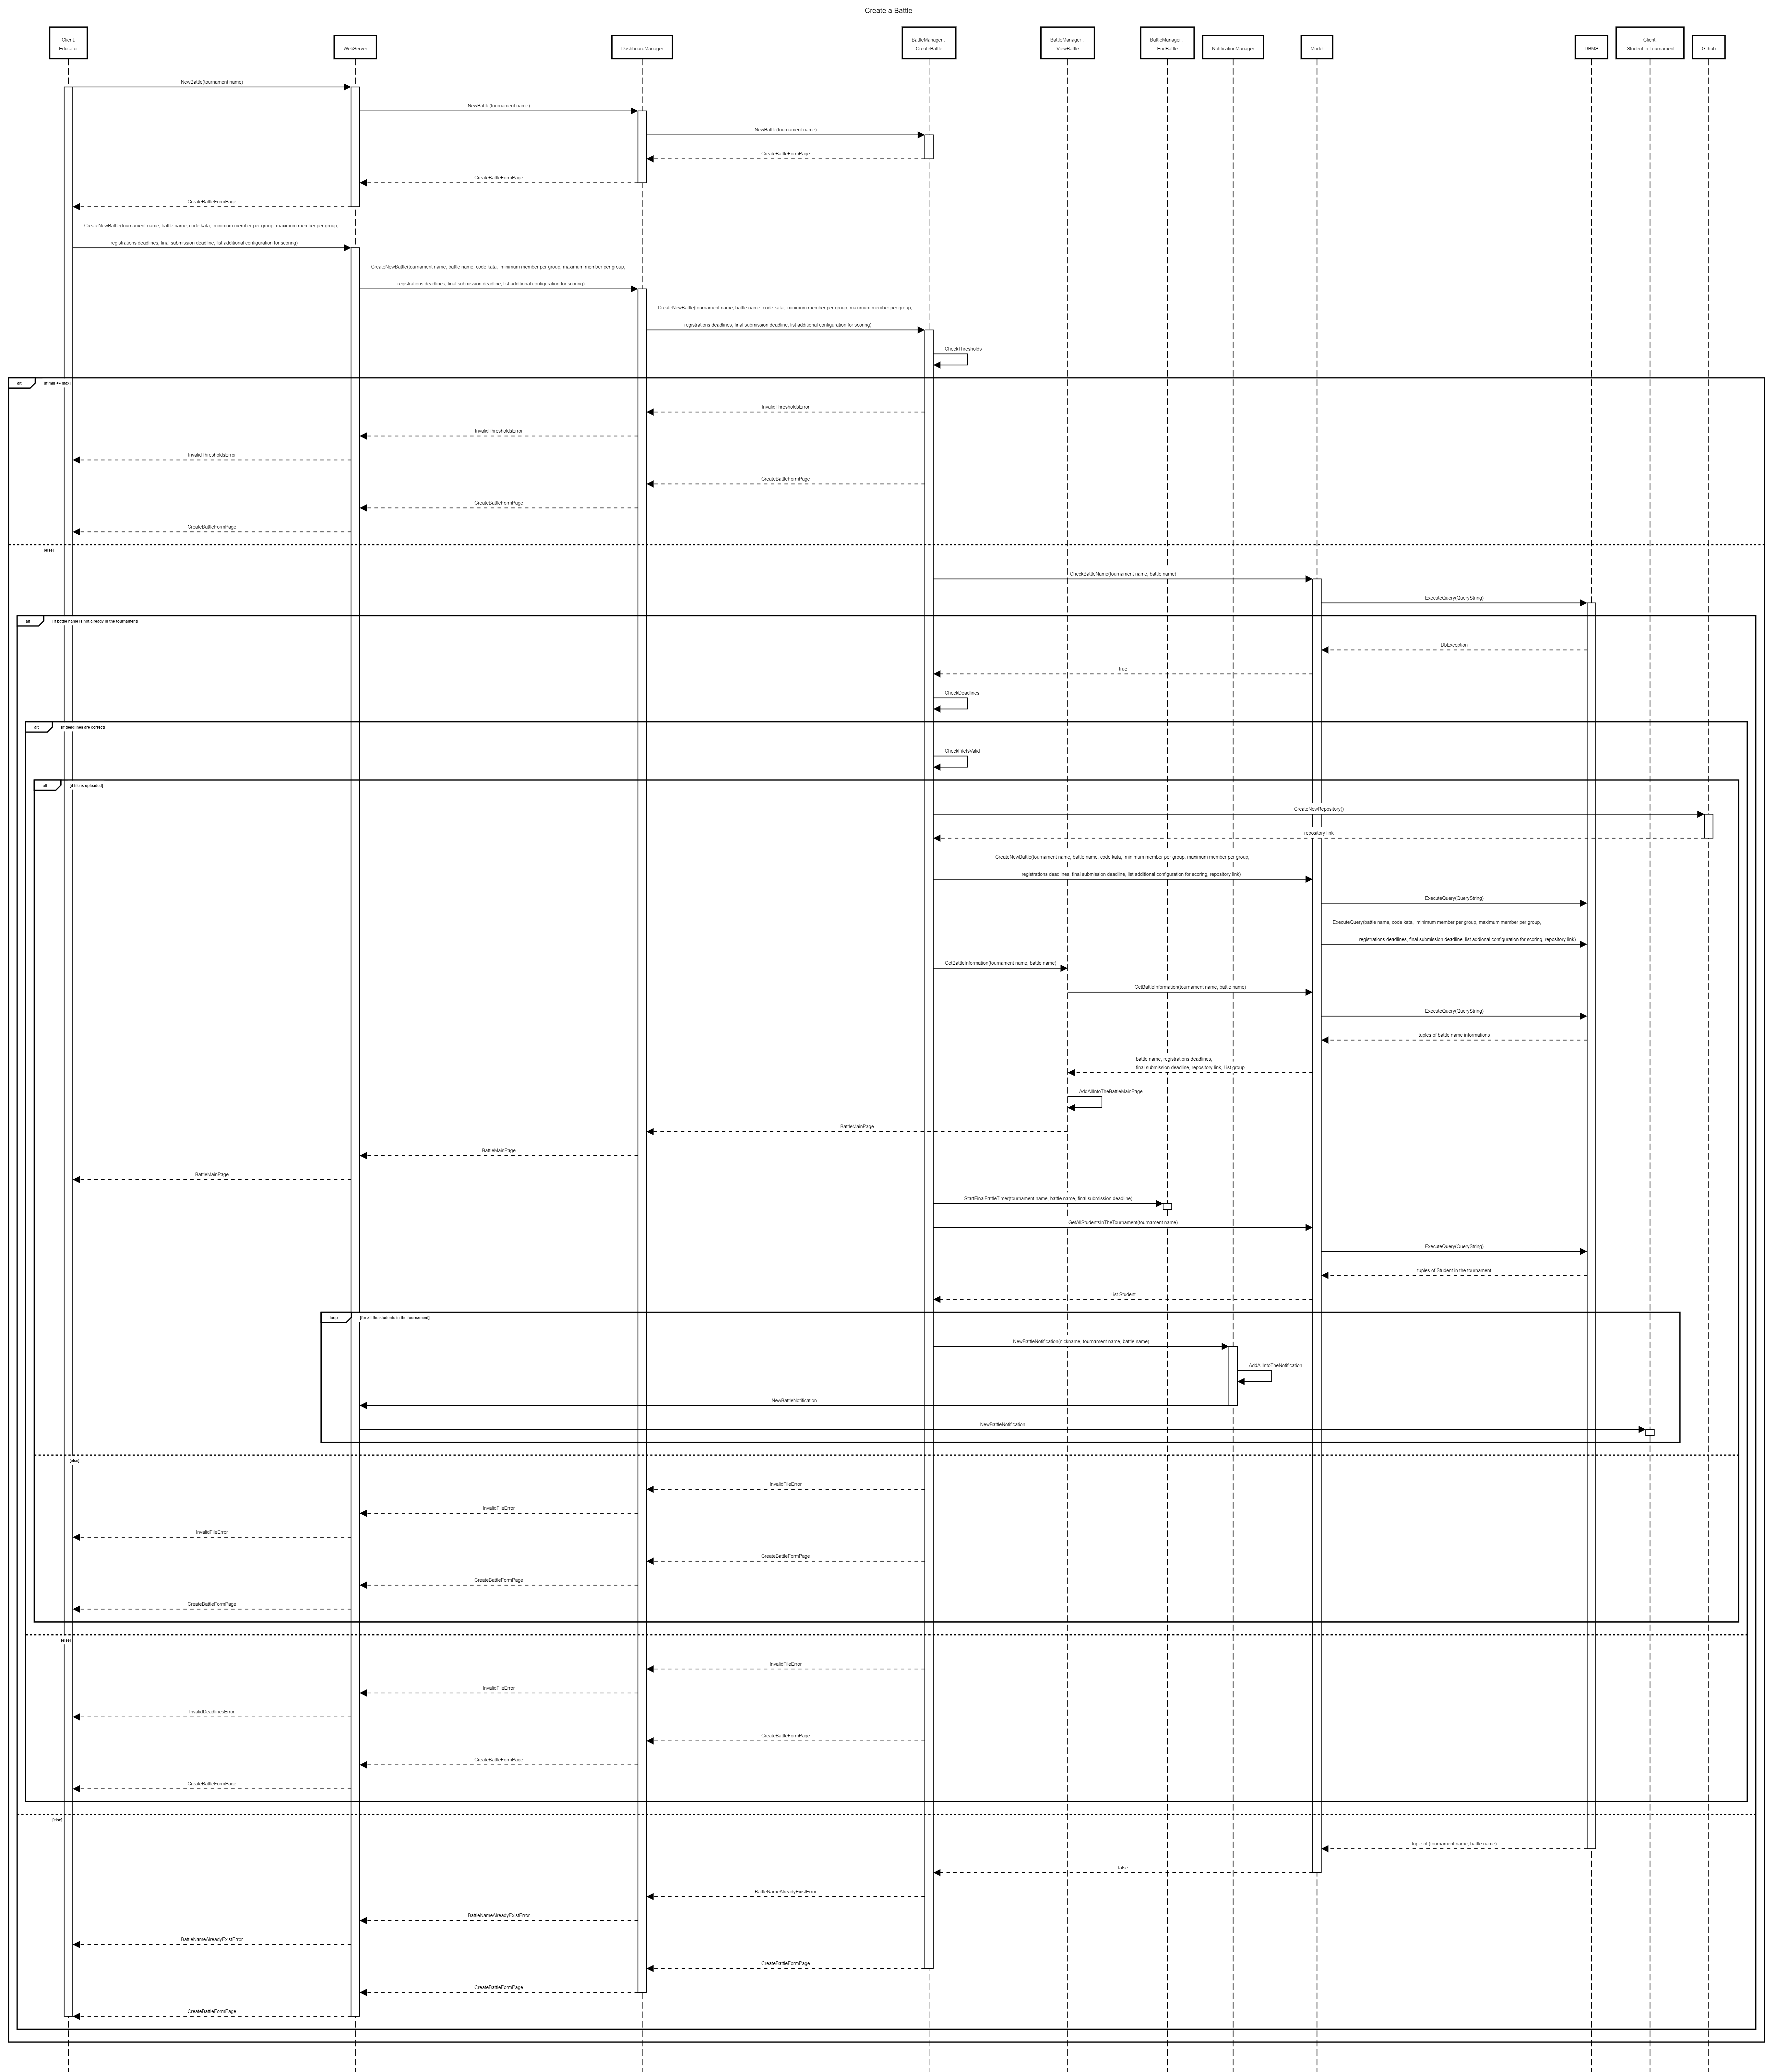
\includegraphics[width=0.8\linewidth]{RuntimeView/CreateBattle.png}
        \caption{Runtime view for 'Create a Battle'.}
        \label{fig:runtime_createbattle}%
    \end{center}
\end{figure}
This sequence diagram represents the flow behind the ‘Battle creation’ 
process. The ED clicks on the “Create a new Battle” button into the “ED Tournament” page. His request is processed by the CreateBattle module that redirects the ED to the Create Battle Form. The ED inserts the new Battle information (Battle name, code kata,  minimum member per group, maximum member per group, registrations deadlines, final submission deadline, list additional configuration for scoring) into the form and sends it to the CreateBattle module. The CreateBattle module does some checks on these informations and if they are all correct he creates a new GH repository and it retrieves the repository link. After this, The CreateBattle module saves the new Battle into the Database (passing through the Model and then the DBMS) and it shows the “ED Battle” page. The CreateBattle module also starts the timer on the EndBattle module and finally it contacts, through the Notification Manager, all the STs in the Tournament to notify them about the start of a new Battle.



\subsection{Join a Battle}
\begin{figure}[H]
    \begin{center}
        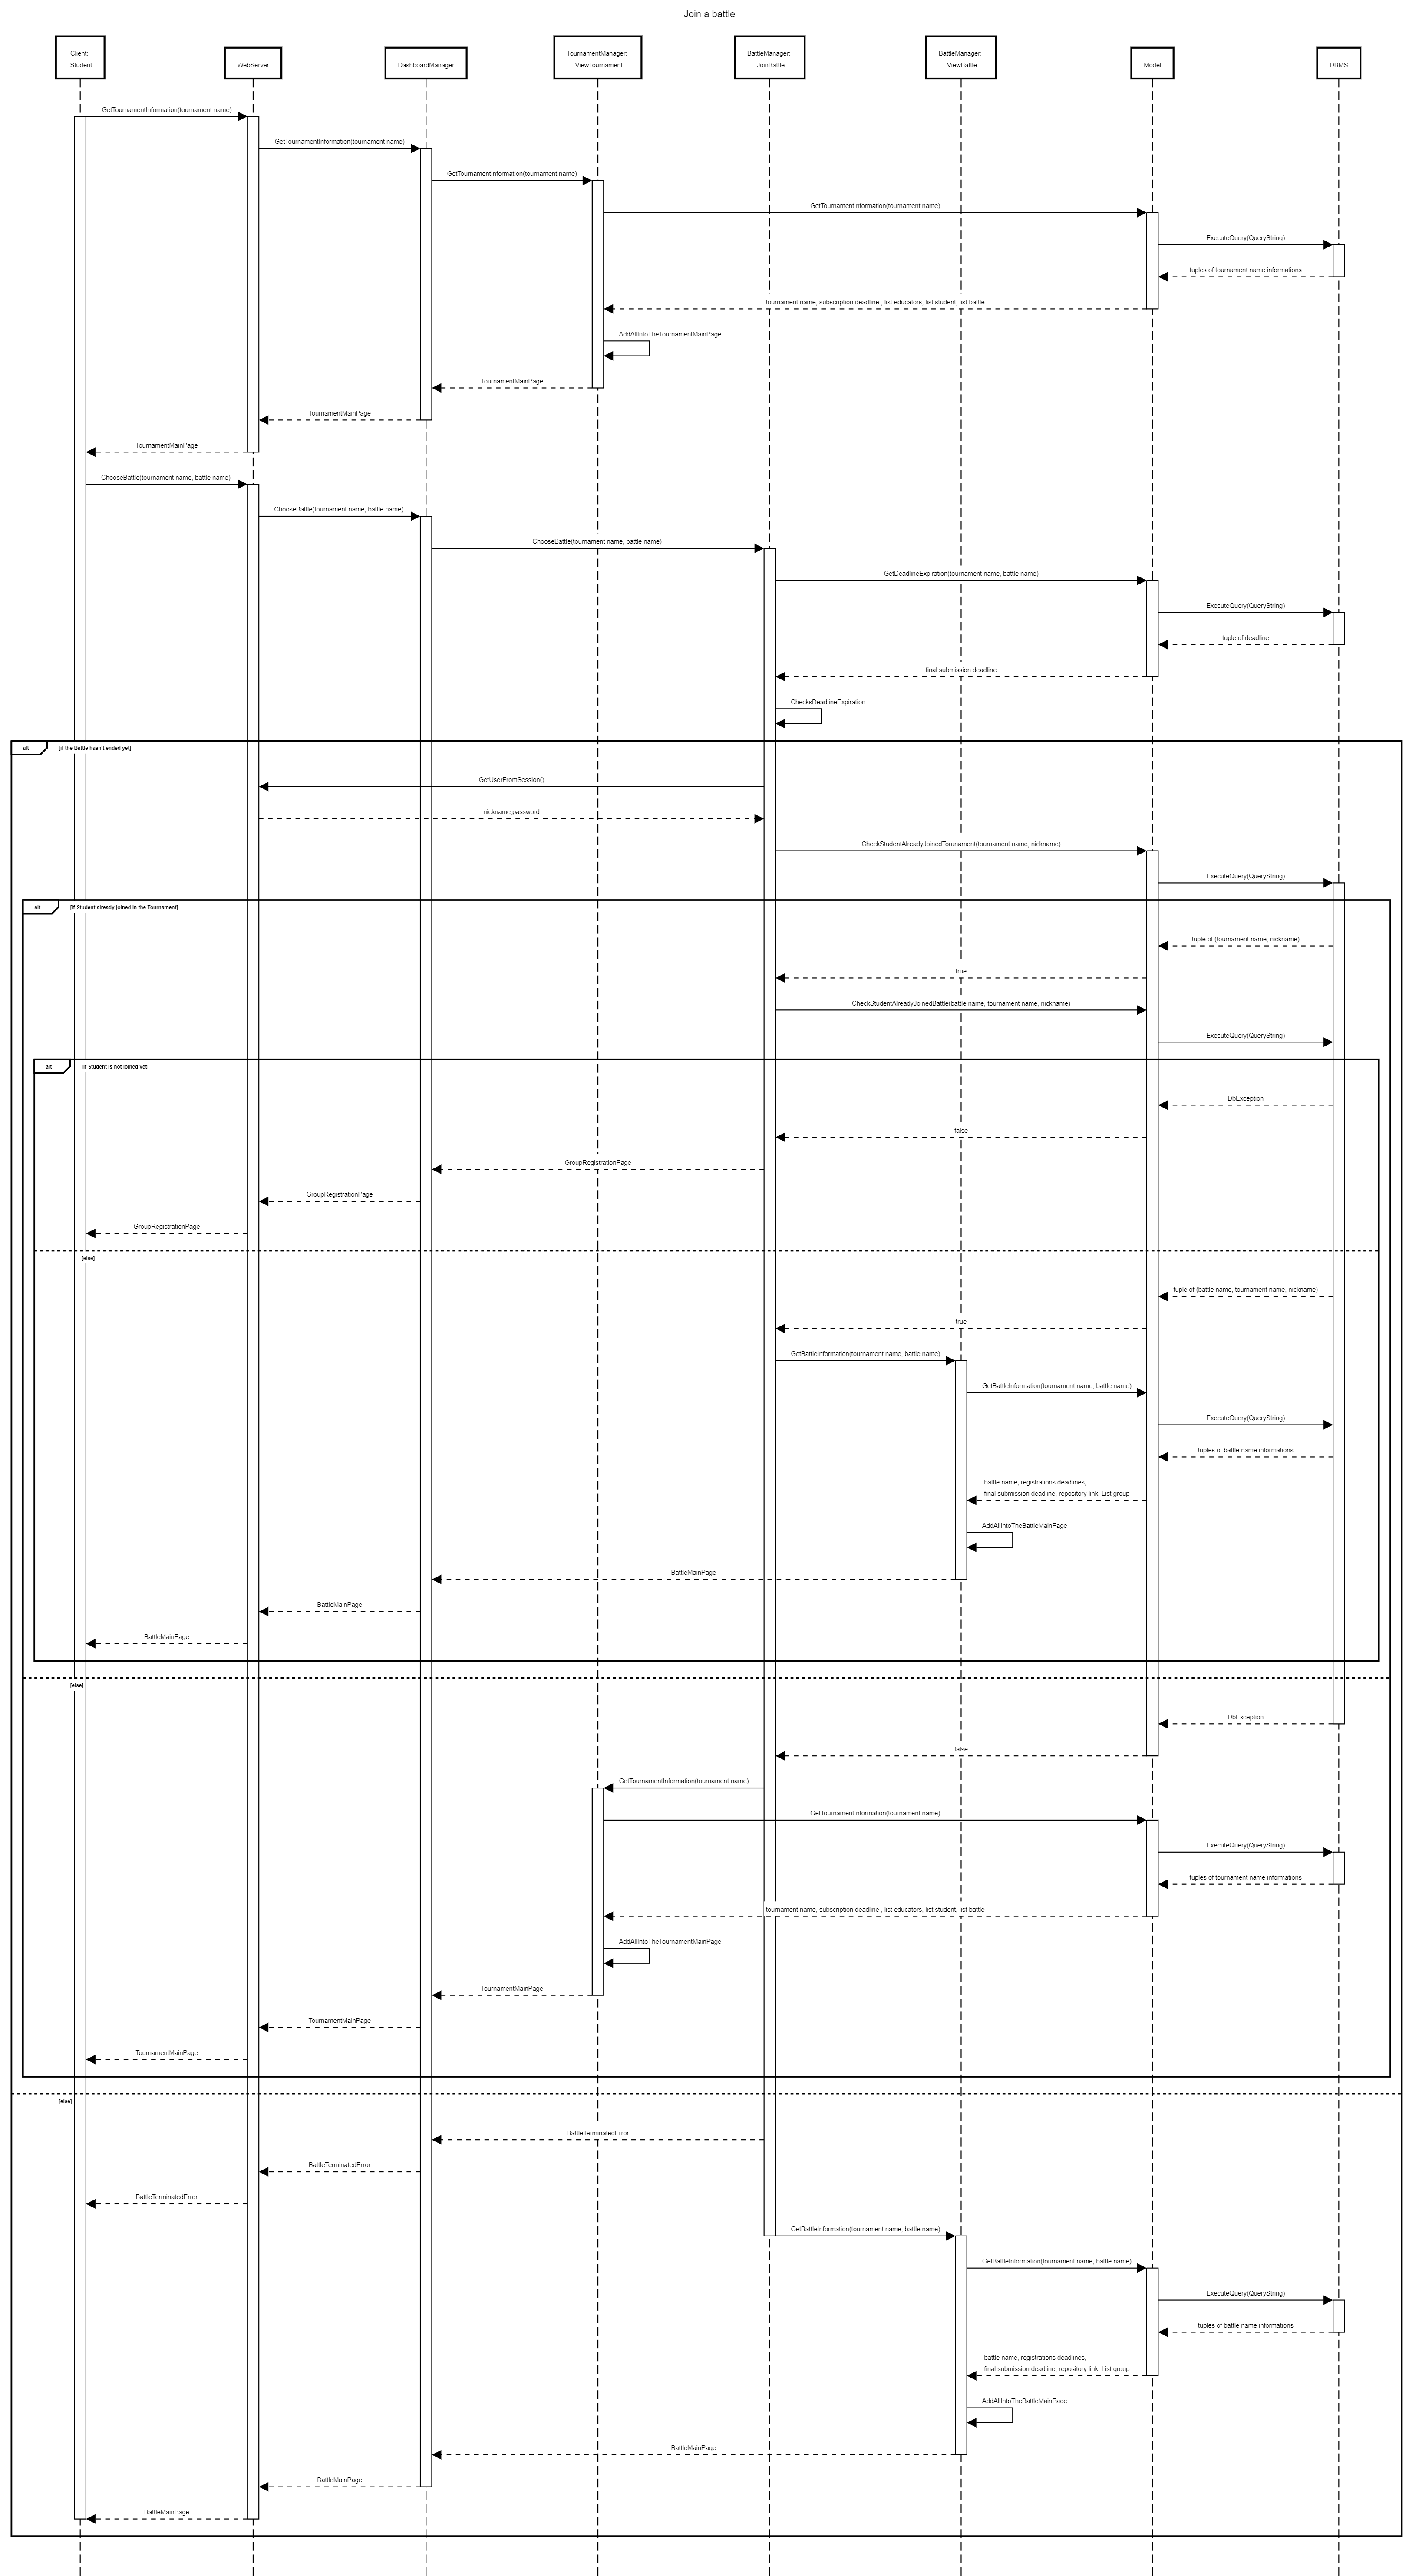
\includegraphics[width=0.8\linewidth]{RuntimeView/JoinBattle.png}
        \caption{Runtime view for 'Join a Battle'.}
        \label{fig:runtime_joinbattle}%
    \end{center}
\end{figure}
This sequence diagram represents the flow behind the ‘Join Battle’ operation for a ST. The ST clicks on a Tournament and the ViewTournament module shows him the “ST Tournament” page. Then the ST clicks on the “Join Battle” button next to the Battle’s name and then the JoinBattle module does the proper checks on the Battle and ST data. If all checks are correct, then the JoinBattle module redirects the ST to the “Create Group” page.


\subsection{Create a group and Battle confirmation}
\begin{figure}[H]
    \begin{center}
        \includegraphics[height=0.8\pdfpageheight]{RuntimeView/CreateGroup.png}
        \caption{Runtime view for 'Create a group and Battle confirmation'.}
        \label{fig:runtime_creategroup}%
    \end{center}
\end{figure}
This sequence diagram represents the flow behind the phase in which, after the fulfillment of the ‘Join Battle’ operations, the ST creates a STG and confirms his participation in the battle.
The ST fills out the Create Group form with some group information (such as group name, list of invited STs nicknames) and then sends it to the CreateGroup module.
The CreateGroup module does some checks on the information coming from the form and then it sends invitations through the Notification Manger to the other STs. If a ST accepts the invitation the CreateGroup module adds the ST to the group and shows to the group creator that the ST has accepted the invitation. If a ST rejects the invitation or if the STG is already full the CreateGroup module shows to the group creator that the ST has rejected the invitation. When the group is formed the ST can click on the “Confirm Group” button and the CreateGroup module adds the group into the Battle and calls the ViewBattle module for showing the Battle main page to the ST.


\subsection{Open a profile}
\begin{figure}[H]
    \begin{center}
        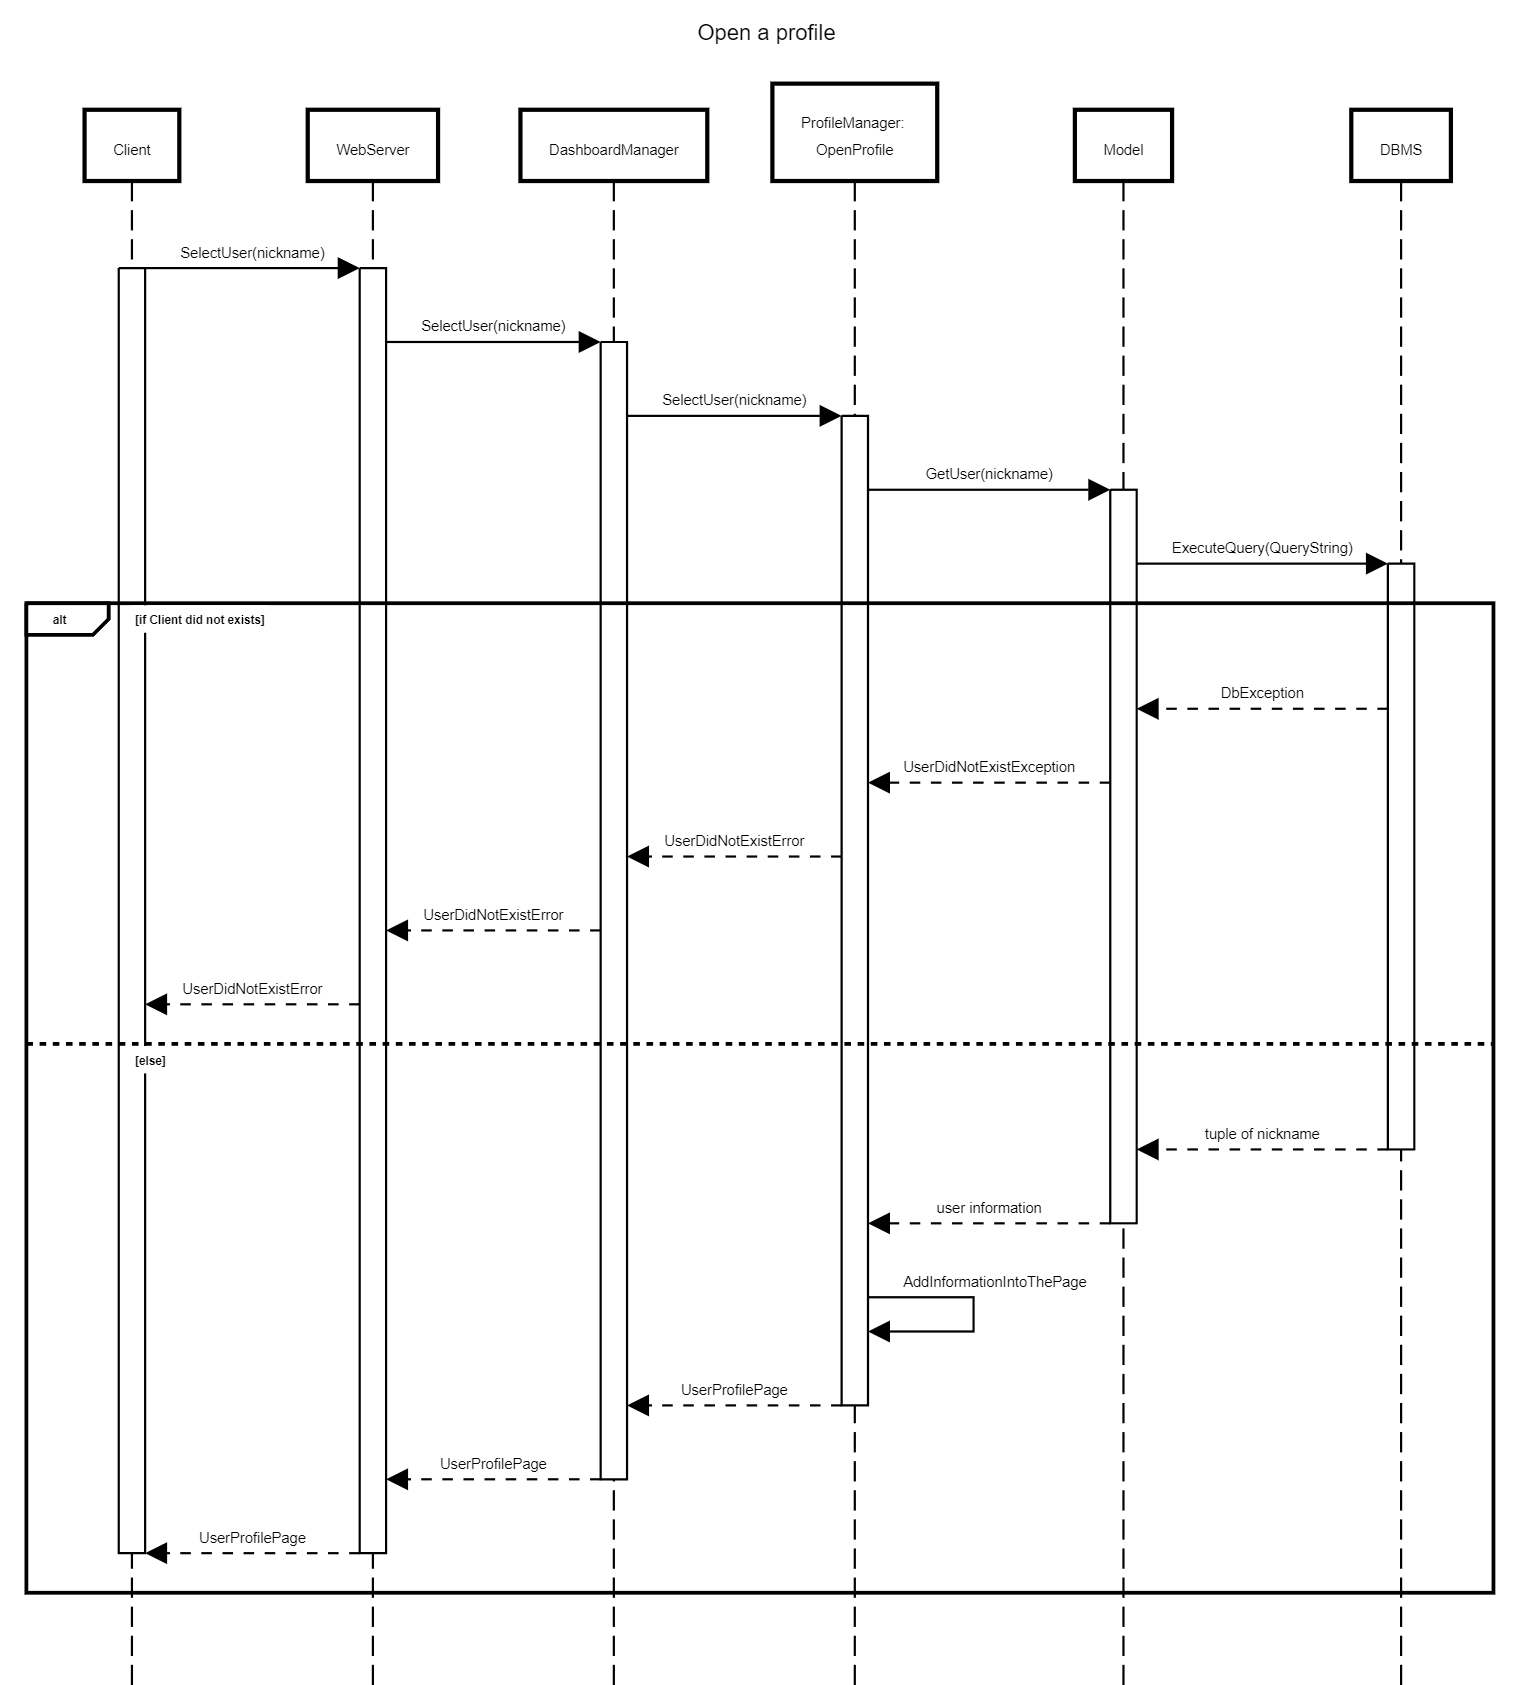
\includegraphics[width=0.8\linewidth]{RuntimeView/OpenProfile.png}
        \caption{Runtime view for 'Open a profile'.}
        \label{fig:runtime_openprofile}%
    \end{center}
\end{figure}
This sequence diagram represents the User open profile process.
The User selects a nickname from the User list and sends it to the DashBoardManager that redirects the request to the OpenProfile module.
The OpenProfile module retrieves from the DBMS the information of the selected User and shows it to the User.


\subsection{Search for a profile}
\begin{figure}[H]
    \begin{center}
        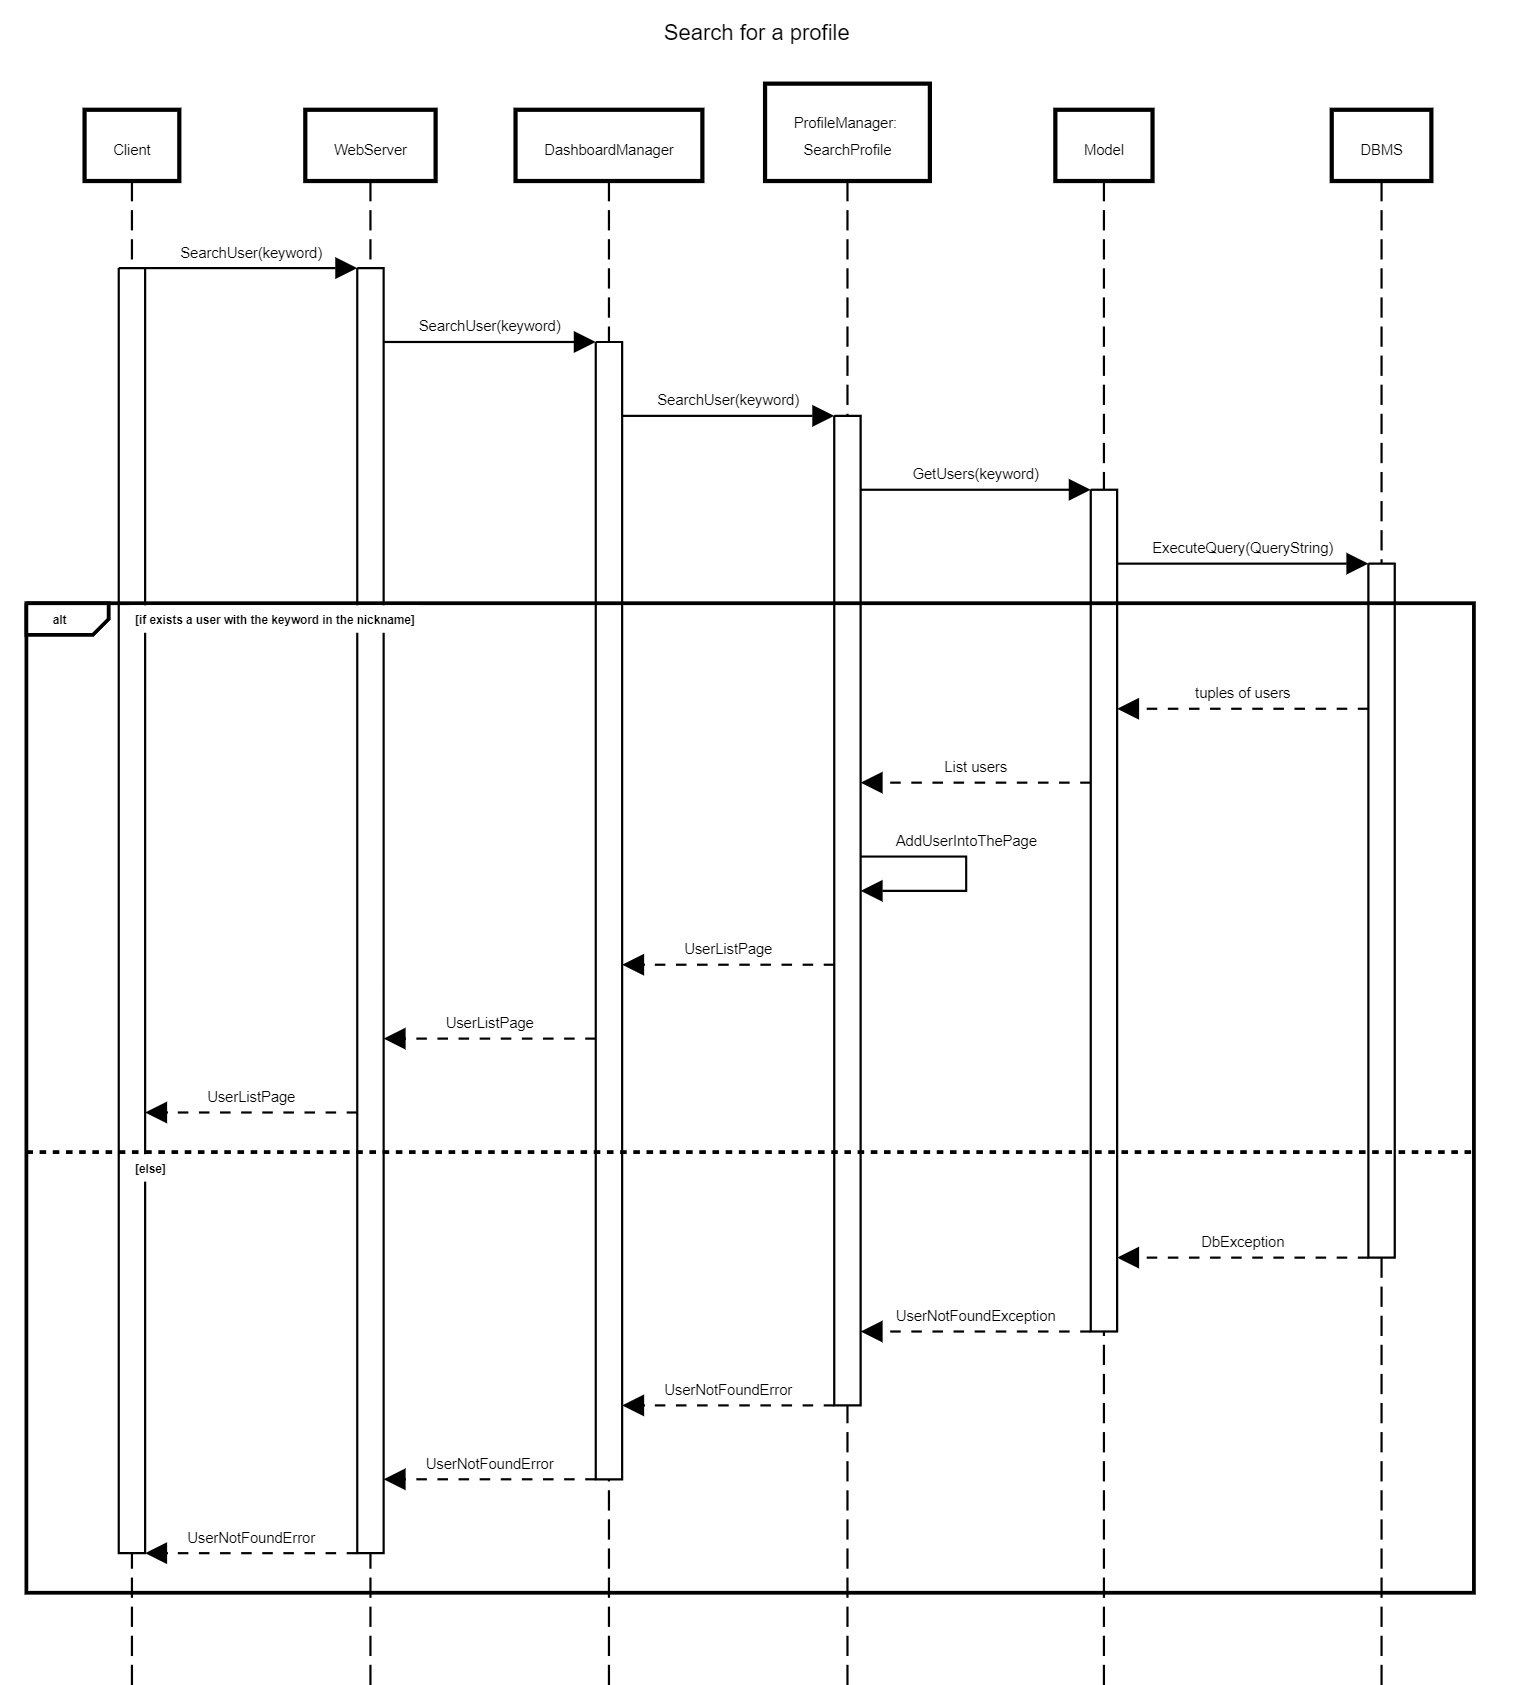
\includegraphics[width=0.8\linewidth]{RuntimeView/SearchProfile.png}
        \caption{Runtime view for 'Search for a profile'.}
        \label{fig:runtime_searchprofile}%
    \end{center}
\end{figure}
This sequence diagram represents the flow behind the profile search.
The User types a keyword into the search bar and sends it to the DashBoardManager that redirects the request to the SearchProfile module.
The SearchProfile module retrieves from the DBMS the list of Users that corresponds to the searched keyword and, if it is not empty, shows it to the User.


\subsection{Search for a Tournament}
\begin{figure}[H]
    \begin{center}
        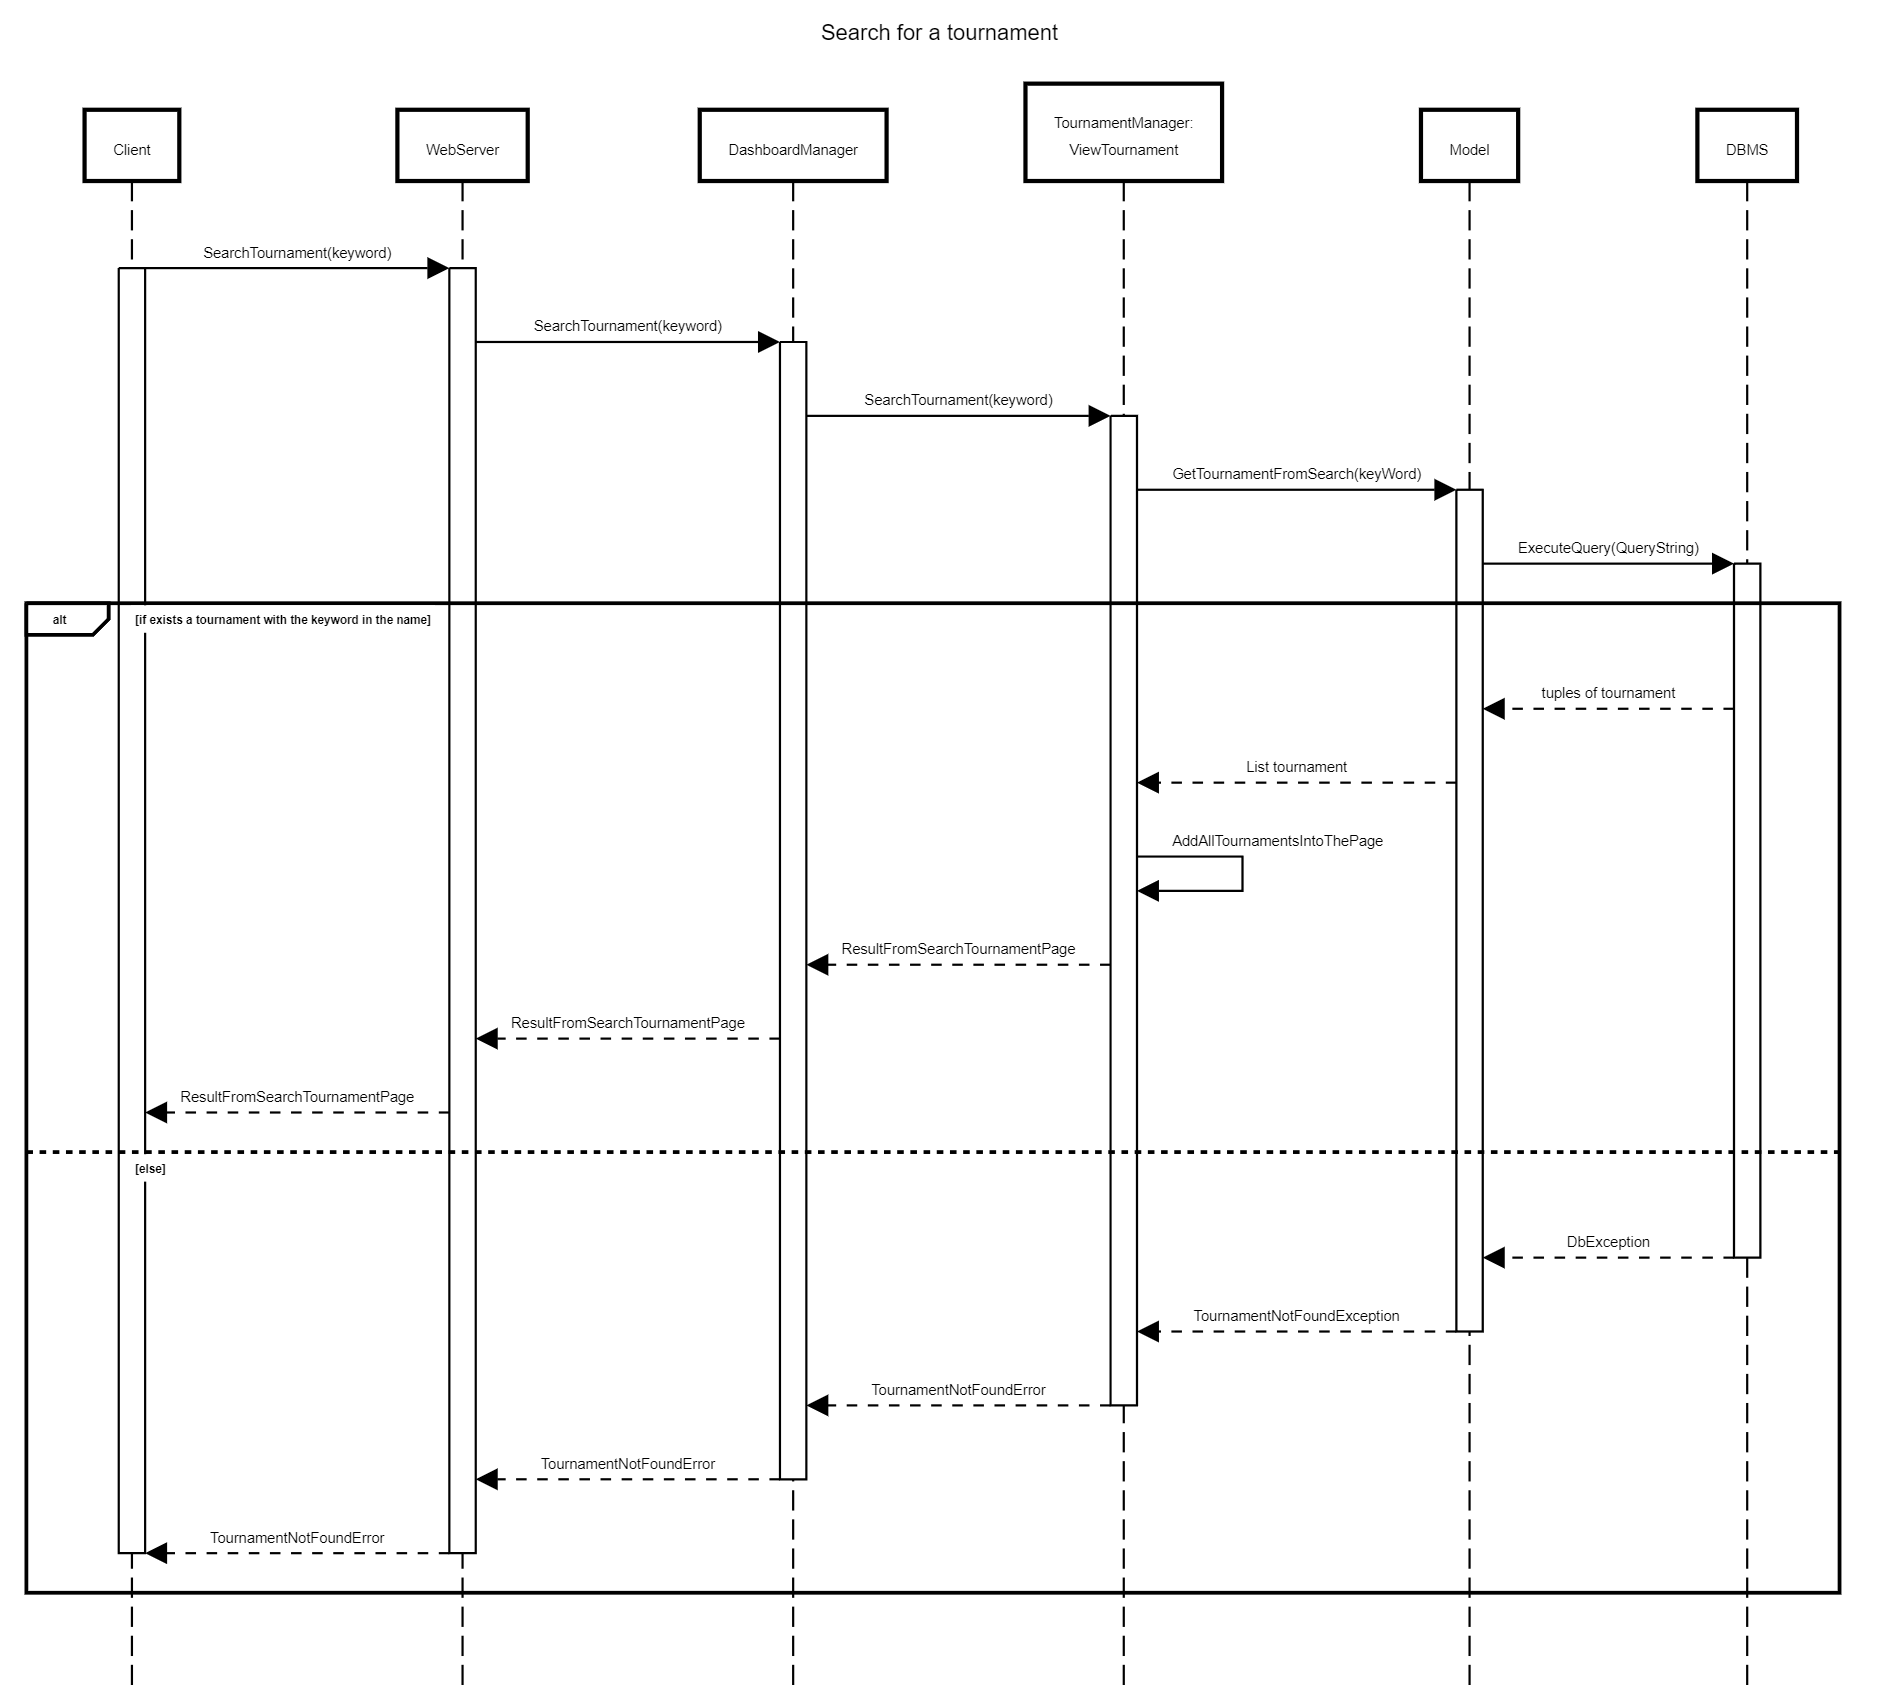
\includegraphics[width=0.8\linewidth]{RuntimeView/SearchTour.png}
        \caption{Runtime view for 'Search for a Tournament'.}
        \label{fig:runtime_searchtournament}%
    \end{center}
\end{figure}
This sequence diagram represents the flow behind the Tournament search.
The User types a keyword into the search bar and sends it to the DashBoardManager that redirects the request to the ViewTournament module.
The ViewTournament module retrieves from the DBMS the list of Tournaments that corresponds to the searched keyword and, if it is not empty, shows it to the User.

\subsection{Evaluate a Code}
\begin{figure}[H]
    \begin{center}
        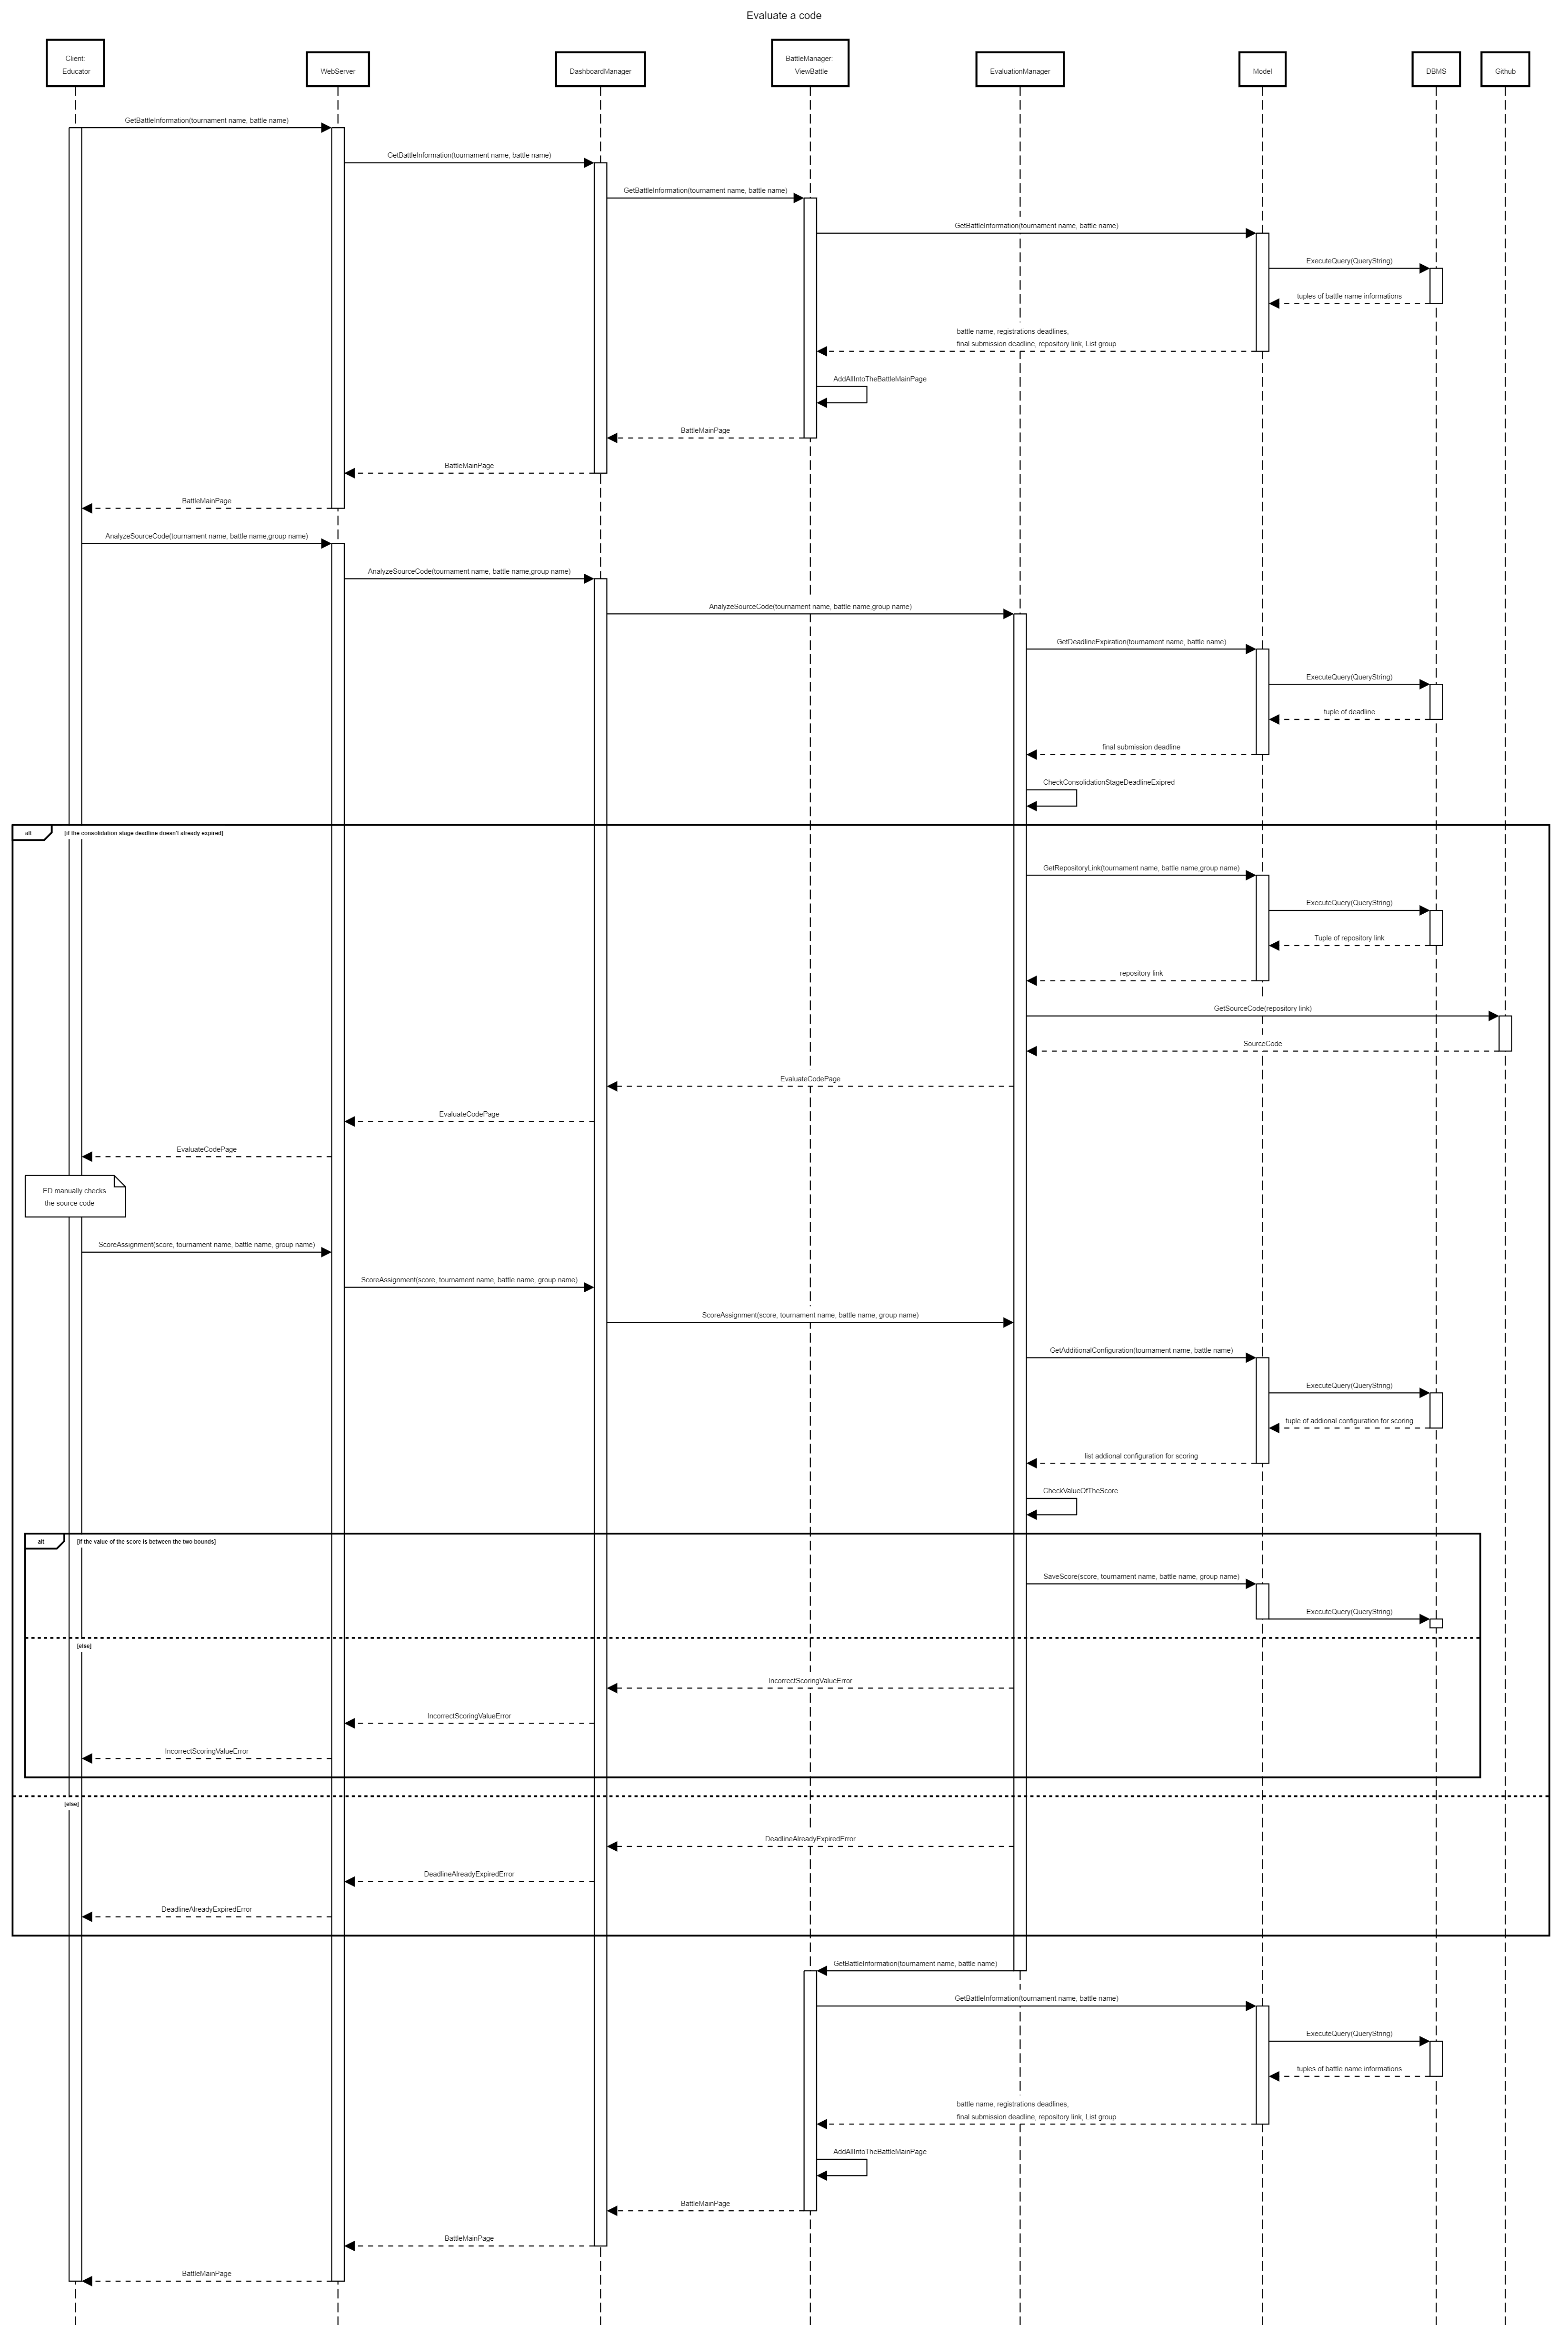
\includegraphics[width=0.8\linewidth]{RuntimeView/EvaluateCode.png}
        \caption{Runtime view for 'Evaluate Code'.}
        \label{fig:runtime_evaluatecode}%
    \end{center}
\end{figure}
This sequence diagram represents the flow behind the ED code evaluation.
The ED clicks on a STG into the ED Battle page and sends his request to the EvaluateManger. The EvaluateManager retrieves the code of that group from GitHub and shows it to the ED. The ED assigns a score to the code and sends it to the EvaluateManger. Finally, the EvaluateManger saves into the Database the score of the STG.

\subsection{Create a new Badge}
\begin{figure}[H]
    \begin{center}
        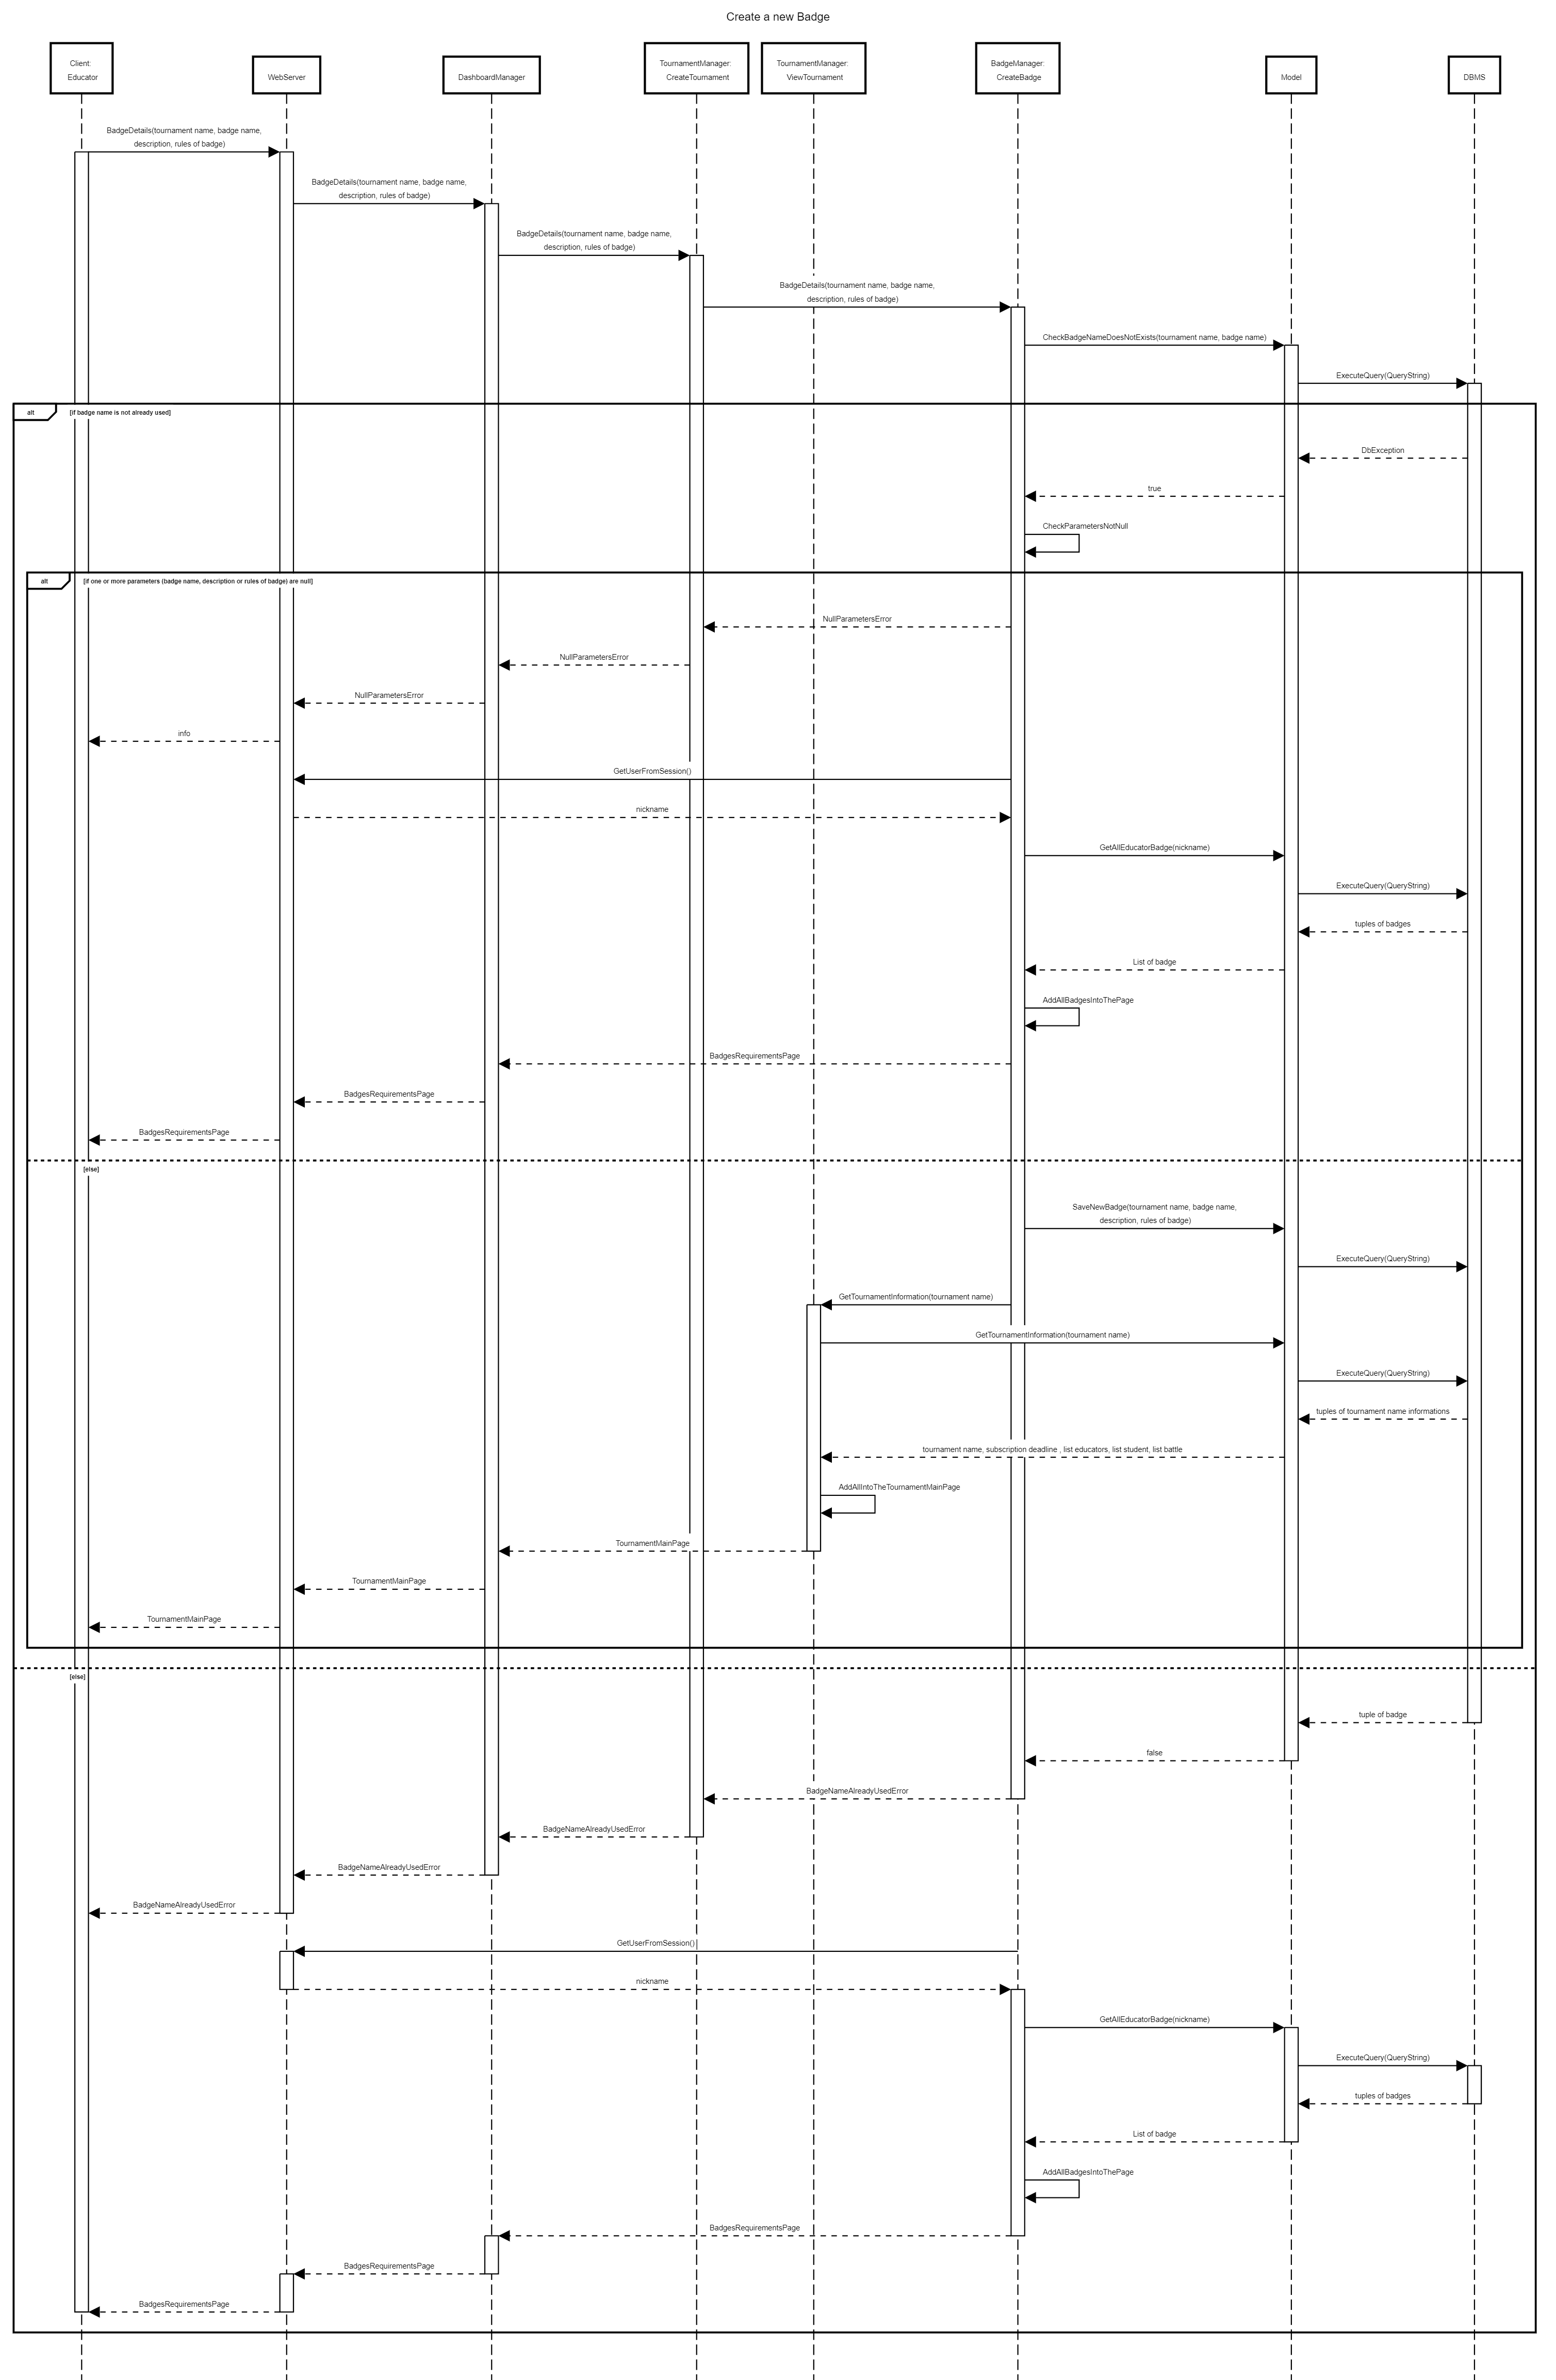
\includegraphics[width=0.8\linewidth]{RuntimeView/CreateBadge.png}
        \caption{Runtime view for 'Create a new Badge'.}
        \label{fig:runtime_createbadge}%
    \end{center}
\end{figure}
This sequence diagram represents the flow behind the creation of a new Badge. The ED inserts into the Create Badge form the information about a new Badge (such as Badge name, description, rules and variables of the Badge) and sends it to the CreateTournament module, which redirects the request to the CreateBadge module. The CreateBadge module checks the new Badge setup and, if they are all correct, saves them into the Database and then calls the ViewTournament module will show the Tournament main page to the ED.

\subsection{Modify an existing Badge}
\begin{figure}[H]
    \begin{center}
        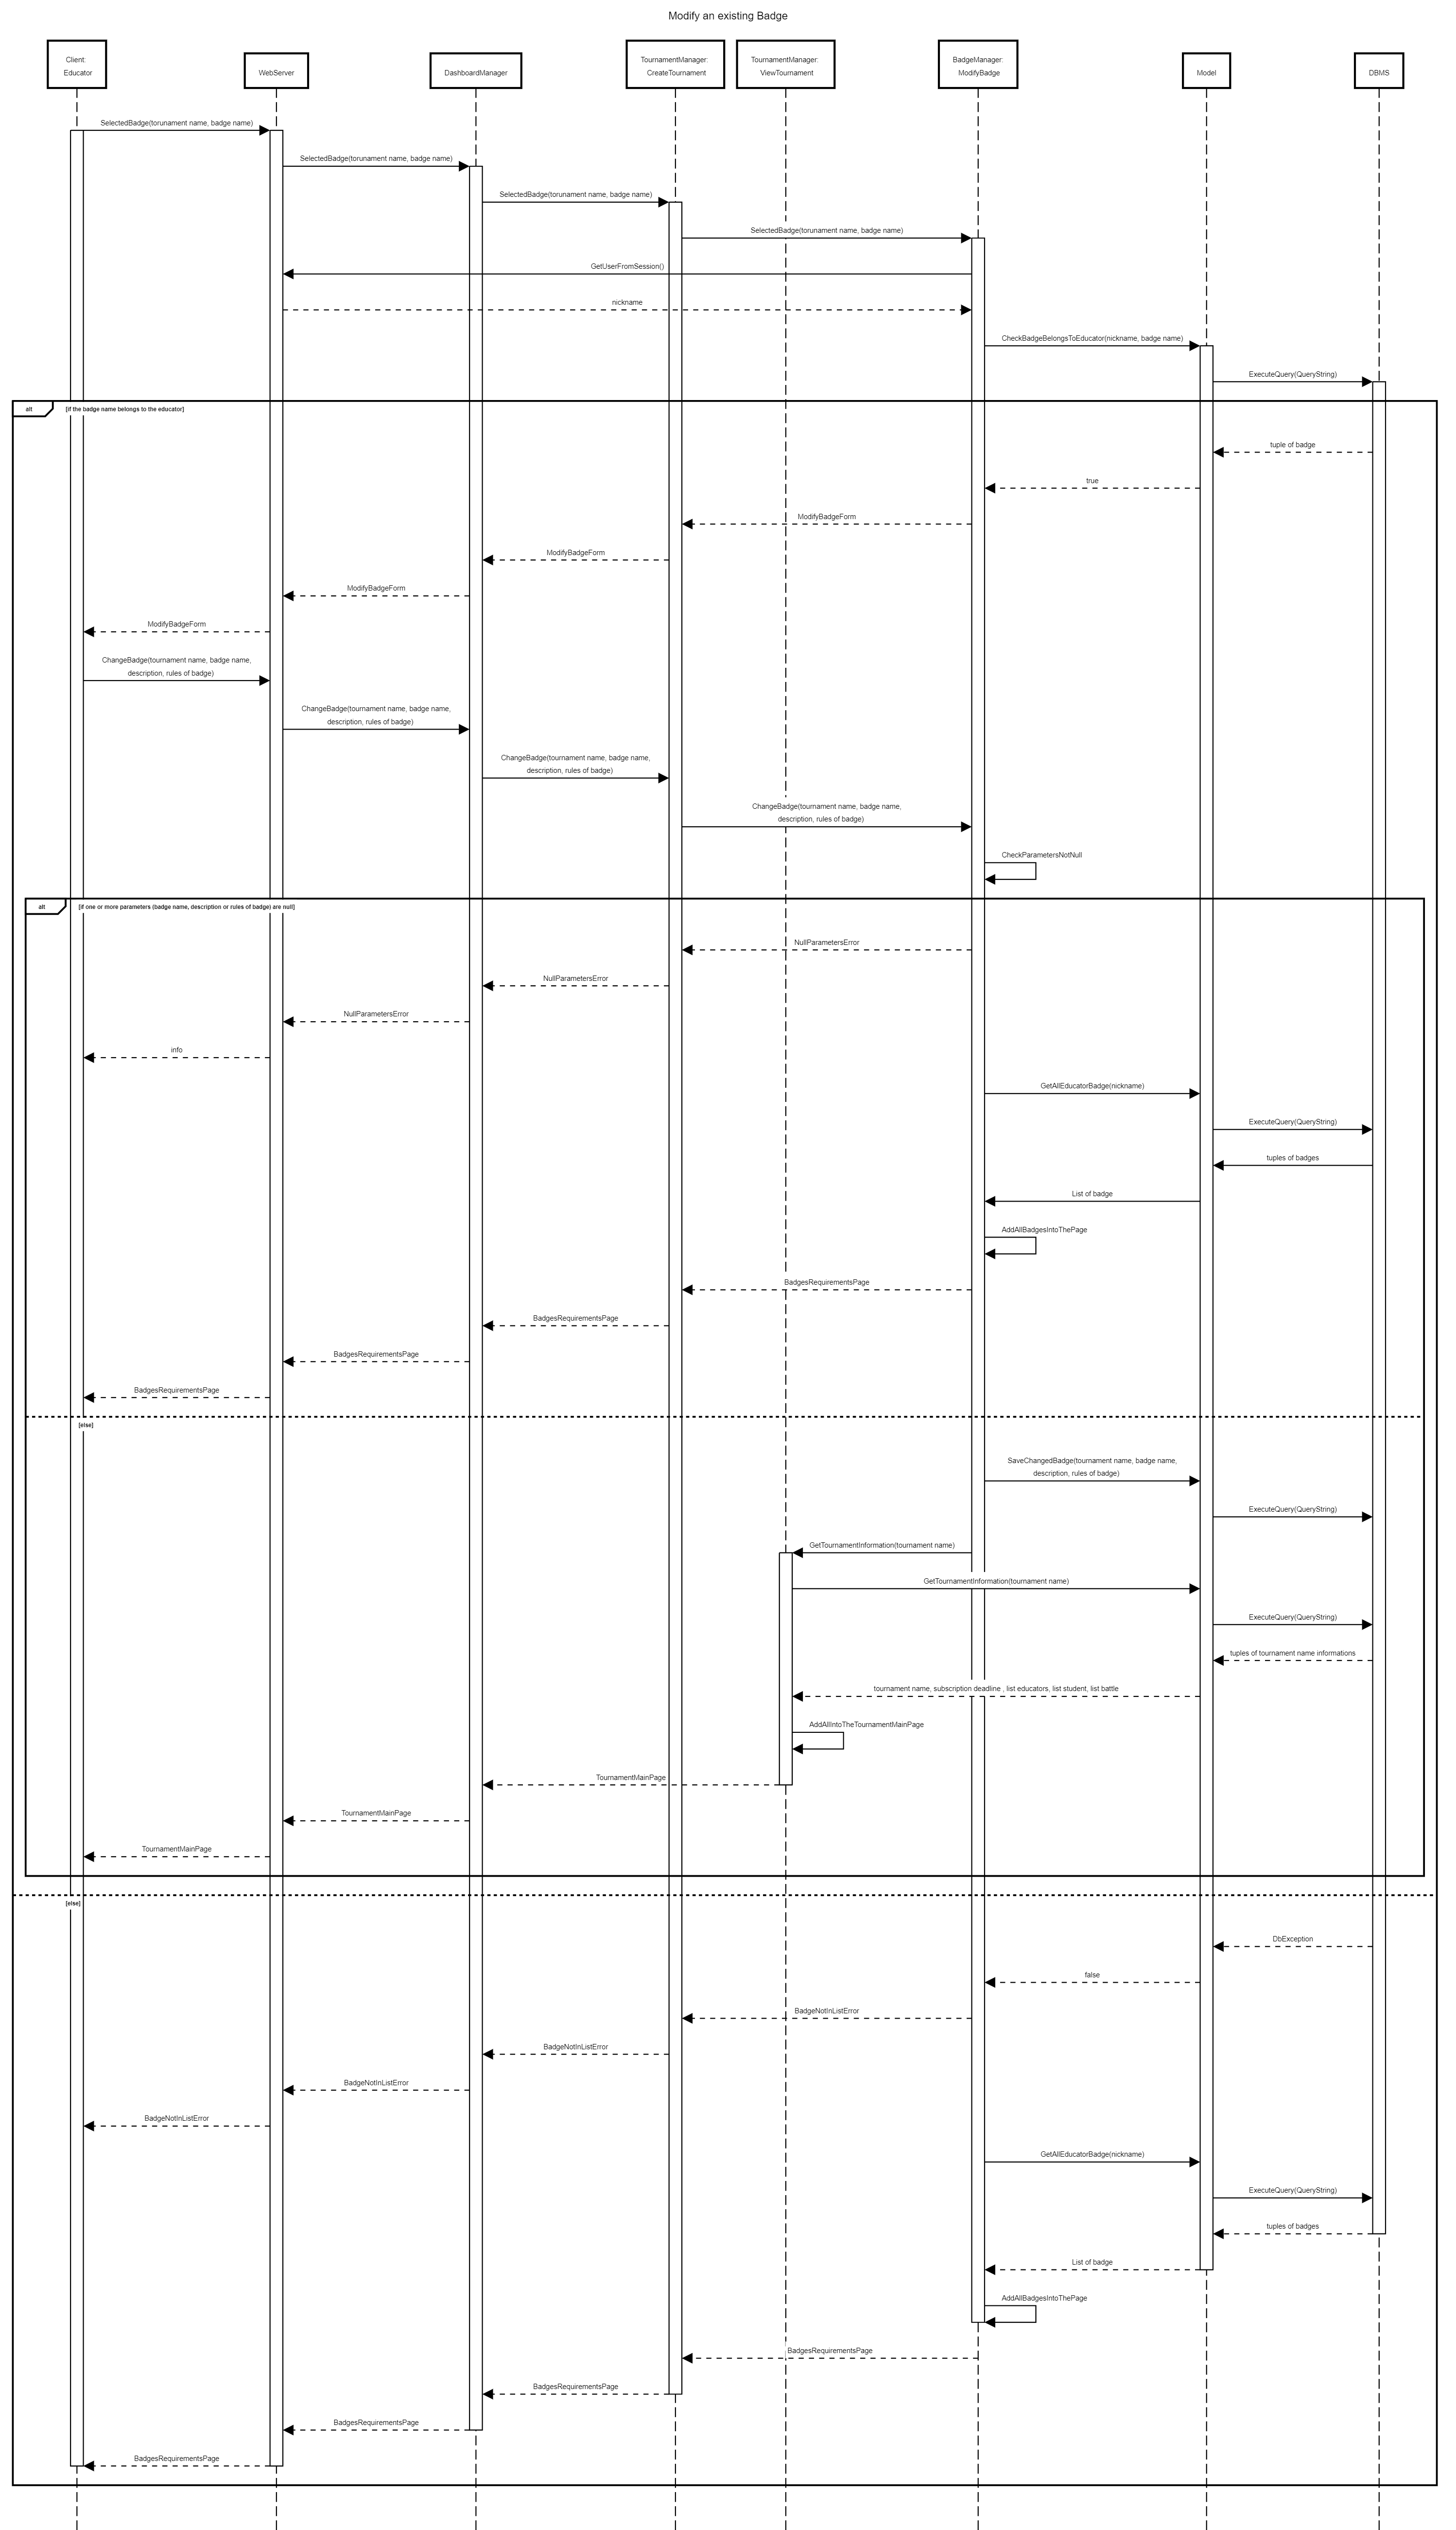
\includegraphics[width=0.8\linewidth]{RuntimeView/ModifyBadge.png}
        \caption{Runtime view for 'Modify an existing Badge'.}
        \label{fig:runtime_modifybadge}%
    \end{center}
\end{figure}
This sequence diagram represents the flow behind the modification of an existing Badge. The ED clicks on an already existing Badge and sends it to the CreateTournament module that redirects the request to the ModifyBadge module that gives to the ED the possibility of changing the badge variables and rules. The ED inserts into the Modify Badge form the new information about the Badge (such as description, rules and variables of the Badge) and sends it to the CreateTournament module, which redirects the request to the ModifyBadge module. The ModifyBadge module checks the new Badge setup and, if they are all correct, saves them into the Database and then calls the ViewTournament module will show the Tournament main page to the ED.





\section{Component Interfaces}
\label{sec:component_interfaces}%
\begin{itemize}
    \item \textbf{\textbf{Login}}
    \begin{itemize}

\item Login(\textit{String} nickname, \textit{String} password)
\end{itemize}
    \item \textbf{\textbf{SearchProfile}}


    \begin{itemize}

\item SearchUser(\textit{String} keyword)
\end{itemize}


    \item \textbf{\textbf{OpenProfile}}
    \begin{itemize}

\item SelectUser(\textit{String} nickname)

\end{itemize}


    \item \textbf{\textbf{RegistrationManager}}

\begin{itemize}
        \item CreateAnAccount()
        \item Registration(\textit{String} name, \textit{String} surname, \textit{String} nickname, \textit{String} mail, \textit{String} password, \textit{Boolean}  ED tick)
        \item Registration(\textit{String} name, \textit{String} surname, \textit{String} nickname, \textit{String} mail, \textit{String} password)
\end{itemize}

    \item \textbf{\textbf{Create Tournament}}

\begin{itemize}
        \item CreateATournament()
        \item TournamentInformation(\textit{String} tournament name, \textit{Date} subscription deadline, \textit{List\textless Educator\textgreater}  list of educators, \textit{Boolean} create badge tick)
        \item BadgeDetails(\textit{String} tournament name, \textit{String} badge name, \textit{String} description, \textit{String} rules of badge)
        \item SelectedBadge(\textit{String} tournament name, \textit{String} badge name)
        \item ChangeBadge(\textit{String} tournament name, \textit{String} badge name, \textit{String} description, \textit{String} rules of badge)
\end{itemize}

    \item \textbf{\textbf{Join Tournament}}
\begin{itemize}
        \item JoinTournament(\textit{String} tournament name)
\end{itemize}

    \item \textbf{\textbf{View Tournament}}

\begin{itemize}
        \item GetTournamentInformation(\textit{String} tournament name)
        \item SearchTournament(\textit{String} keyword)
\end{itemize}

    \item \textbf{\textbf{CreateBadge}}
\begin{itemize}

    \item BadgeDetails(\textit{String} tournament name, \textit{String} badge name, \textit{String} description, \textit{String} rules of badge)
\end{itemize}

    \item \textbf{\textbf{ModifyBadge}}

\begin{itemize}
        \item SelectedBadge(\textit{String} tournament name, \textit{String} badge name)
        \item ChangeBadge(\textit{String} tournament name, \textit{String} badge name, \textit{String} description, \textit{String} rules of badge)
\end{itemize}

    \item \textbf{\textbf{Model}}

\begin{itemize}
        \item CheckCredentials(\textit{String} nickname, \textit{String} password)
        \item GetEducatorTournaments(\textit{String} nickname)
        \item GetStudentTournaments(\textit{String} nickname)
        \item GetNewBattlesFromTournaments(\textit{List\textless Tournament\textgreater} list tournament, \textit{String} nickname)
        \item GetLastTournaments()
        \item GetRepositoryLink(\textit{String} tournament name, \textit{String} battle name, \textit{String} group name)
        \item GetAdditionalConfiguration(\textit{String} tournament name, \textit{String} battle name)
        \item SaveScore(\textit{Int}  score, \textit{String} tournament name, \textit{String} battle name, \textit{String} group name)
        \item CheckNickname(\textit{String} nickname)
        \item CheckMail(\textit{String} mail)
        \item SaveNewUserCredentials(\textit{String} name, \textit{String} surname, \textit{String} nickname, \textit{String} mail, \textit{String} password, \textit{Boolean}  ED tick)
        \item GetAllStudents()
        \item GetUser(\textit{String} nickname)
        \item GetUsers(\textit{String} keyword)
        \item GetDeadlineExpiration(\textit{String} tournament name)
        \item GetDeadlineExpiration(\textit{String} tournament name, \textit{String} battle name)
        \item GetRegistrationDeadline(\textit{String} tournament name, \textit{String} battle name)
        \item CheckBadgeNameDoesNotExists(\textit{String} tournament name, \textit{String} badge name)
        \item GetAllEducatorBadge(\textit{String} nickname)
        \item SaveNewBadge(\textit{String} tournament name, \textit{String} badge name, \textit{String} description, \textit{String} rules of badge)
        \item CheckBadgeBelongsToEducator(\textit{String} nickname, \textit{String} badge name)
        \item SaveChangedBadge(\textit{String} tournament name, \textit{String} badge name, \textit{String} description, \textit{String} rules of badge)
        \item GetTournamentName(\textit{String} tournament name)
        \item GetTournamentInformation(\textit{String} tournament name)
        \item GetTournamentFromSearch(\textit{String} keyWord)
        \item GetStudentTournaments(\textit{String} nickname)
        \item GetLastTournaments()
        \item SaveStudentAsTournamentPartecipant(\textit{String} tournament name, \textit{String} nickname)
        \item GetAllStudentsIntheTournament(\textit{String} tournament name)
        \item CheckStudentAlreadyJoinedTournament(\textit{String} tournament name, \textit{List\textless String\textgreater} list nicknames)
        \item CheckStudentAlreadyJoinedTouenament(\textit{String} tournament name, \textit{String} nickname)
        \item CheckGroupAlreadyJoined(\textit{String} tournament name, \textit{String} battle name, \textit{String} group name)
        \item CheckGroupNumber(\textit{String} tournament name, \textit{String} battle name, \textit{String} group name)
        \item SaveGroupIntheBattleList(\textit{String} tournament name, \textit{String} battle name, \textit{String} group name)
        \item CheckBattleName(\textit{String} tournament name, \textit{String} battle name)
        \item GetBattleInformation(\textit{String} tournament name, \textit{String} battle name)
        \item CheckGroupName(\textit{String} tournament name, \textit{String} battle name, \textit{String} group name)
        \item CheckGroupParticipants(\textit{String} tournament name, \textit{String} battle name, \textit{String} group name)
        \item AddStudentToGroup(\textit{String} nickname, \textit{String} tournament name, \textit{String} battle name, \textit{String} group name)
        \item CreateNewBattle(\textit{String} tournament name, \textit{String} battle name, \textit{String} code kata, \textit{Int}  minimum member per group, \textit{Int}  maximum member per group, \textit{Date} registration deadline, \textit{Date} final submission deadline, \textit{List\textless String\textgreater} list additional configuration for scoring, \textit{String} repository link)
        \item CheckStudentAlreadyJoinedBattle(\textit{String} battle name, \textit{String} tournament name, \textit{String} nickname)
        \item GetEducatorsName(\textit{List\textless Educators\textgreater} list of educators)
        \item SaveNewTournament(\textit{String} tournament name, \textit{String} subscription deadline, \textit{List\textless Educators\textgreater} list of educators)
\end{itemize}

    \item \textbf{\textbf{CreateBattle}}

\begin{itemize}
        \item NewBattle(\textit{String} tournament name)
        \item CreateBattle(\textit{String} battle name, \textit{String} code kata, \textit{Int}  minimum member per group, \textit{Int}  maximum member per group, \textit{Date} registration deadline, \textit{Date} final submission deadline, \textit{List\textless String\textgreater} list additional configuration for scoring)
\end{itemize}

\end{itemize}

\begin{itemize}
    \item \textbf{\textbf{JoinBattle}}
\begin{itemize}
    \item ChooseBattle(\textit{String} tournament name, \textit{String} battle name)
    \end{itemize}


    \item \textbf{\textbf{CreateGroup}}

\begin{itemize}
        \item CreateGroupAndInvitation(\textit{String} tournament name, \textit{String} battle name, \textit{String} group name, \textit{List\textless String\textgreater} list nicknames)
        \item acceptInvitation(Student student, \textit{String} tournament name, \textit{String} battle name, \textit{String} group name)
        \item rejectInvitation(Student student, \textit{String} tournament name, \textit{String} battle name, \textit{String} group name)
        \item JoinBattle(\textit{String} tournament name, \textit{String} battle name, \textit{String} group name)
\end{itemize}

    \item \textbf{\textbf{ViewBattle}}
    \begin{itemize}
        \item GetBattleInformation(\textit{String} tournament name, \textit{String} battle name)
\end{itemize}

    \item \textbf{\textbf{EndBattle}}
\begin{itemize}
        \item StartFinalBattleTimer(\textit{String} tournament name, \textit{String} battle name, \textit{Date} final submission deadline)
\end{itemize}

    \item \textbf{\textbf{NotificationManager}}

\begin{itemize}
        \item ChosenEducatorNotification(\textit{String} nickname, \textit{String} tournament name)
        \item NewBattleNotification(\textit{String} nickname, \textit{String} tournament name, \textit{String} battle name)
        \item NewTournamentNotification(\textit{String} nickname, \textit{String} tournament name)
        \item SendInvitation(\textit{String} nickname, \textit{String} tournament name, \textit{String} battle name, \textit{String} group name)
\end{itemize}

    \item \textbf{\textbf{EvaluationManager}}

\begin{itemize}
        \item AnalyzeSourceCode(\textit{String} tournament name, \textit{String} battle name, \textit{String} group name)
        \item ScoreAssignment(\textit{Int}  score, \textit{String} tournament name, \textit{String} battle name, \textit{String} group name)
\end{itemize}

    \item \textbf{\textbf{DashboardManager}} (contains all the interfaces belonging to other managers, apart from NotificationManager and Model)

    \item \textbf{\textbf{WebServer}} (contains all the interfaces belonging to other managers, apart from NotificationManager and Model)
    \begin{itemize}
        \item GetSessionFromUser()
        \item AddUserToTheSession(\textit{String} nickname, \textit{String} password)
\end{itemize}

\end{itemize}


\section{Selected Architectural Styles and Patterns}
\label{sec:selected_Srchitectural_styles_patterns}%

CodeKataBattle will be developed over a \textbf{3-Tier architecture}, which is a software application architecture that organizes applications into three logical and physical computing tiers. Each tier runs on its own infrastructure, so the complexity of the system is reduced, its flexibility and scalability is enhanced. Each tier may be developed simultaneously by separate teams of developers and can be updated or scaled as needed without impacting the other tiers.
\\
The system is modularized over three independent tiers:
\begin{itemize}
    \item \textbf{Presentation Tier:} this is the top-level tier, that directly interacts with the Users. Its goal will be to collect the Users’ inputs and show them the outputs produced by the lower tiers. 
    \item \textbf{Application Tier:} this is the middle level tier. The Application Tier processes the Users’ requests that arrive from the Presentation Tier, perform the necessary computation, even retrieving or storing data on the Data Tier, and computes that data in order to complete specific tasks requested by the Users. This tier needs to handle several requests by different Users simultaneously, while guaranteeing the security and integrity of the stored data.
    \item \textbf{Data Tier:} this is the lowest level tier. The Data Tier stores, retrieves and manages data used or produced by the Application Tier by the DataBase System’s APIs.
\end{itemize}

For a more detailed description of the tiers and their components, please refer to \ckbautoref{sec:deployment_view}.\\
The behavior of the system will be mostly as a \textbf{Client-Server architecture}, in which the Client represents the front-end user interface, as it is the connection point between the final Users of the system and the system itself, meanwhile the Server represents the backend platform, as it elaborates the Users’ requests, computes and shows the answers. In a pure Client-Server architecture, the Server is always the one to make the request, while the server is a passive element, which handles and elaborates the requests of the Client and returns the answers to them. In some cases, such as when the process of sending the notifications or the interaction with the External Tools, the Server needs to perform operations without being invoked by the Client first, which makes it an active component and having a more Event Driven behavior.
\\
The Client-Server interactions are performed through \textbf{REST APIs}, a set of commands commonly used in the context of web transactions. The \textit{Representational State Transfer} consists in the use of a stateless Server, that means that the Client is the component that needs to communicate the state of the transaction to the Server. This approach allows the Server to be more scalable and helps with handling many requests that concern different states simultaneously. The components communicate by transferring a representation of a resource in a format that the Server is able to process, this allows the usage of HTTP protocol to share data and to encode those using the JSON format.
\\
The implementation of CKB will follow the \textbf{Model-View-Controller} pattern, which is a software design pattern that splits the software into three elements interconnected with each other: 
\begin{itemize}
    \item \textbf{Model:} contains the methods that manage the data. It provides methods for saving, retrieving and manipulating data from the database.
    \item \textbf{View:} the view is the part that concerns the visual representation of the data for the final user.
    \item \textbf{Controller:} acts as a connection point between the view and the model. The controller handles the users’ interactions with the view and processes the operations.
\end{itemize}

\section{Other Design Decisions}
\label{sec:other_design_decisions}%

\subsection{Availability}
The introduction of load balancing and replication mechanisms significantly enhances the reliability and availability of our system. Load balancing optimizes resource utilization by distributing requests evenly across servers, preventing performance bottlenecks.\\ Concurrently, replication ensures fault tolerance by duplicating essential data and services. This redundancy minimizes the impact of potential failures, fortifying our system to maintain consistent data management and service availability even in challenging scenarios.

\subsection{Scalability}
Microservices architecture, at its core, is meticulously crafted to be both independently deployable and inherently scalable. This design philosophy enables each microservice to be deployed autonomously, facilitating swift updates and modifications without disrupting the entire system. Beyond this, the scalability aspect of microservices empowers our system to gracefully handle increased demands by efficiently scaling specific services.


\subsection{Notification Handling}
Notification management plays a pivotal role in the CKB system, influencing every stage from Tournament, Battle or STG creation to their conclusion. Notifications in CKB are orchestrated to reach users upon login or, if a User is already logged in, immediately when they become available. This approach guarantees that Users are promptly informed about key events, such as Tournament, Battle or STG creation. 

\subsection{Ease of Deployment} 
The adoption of microservices architecture introduces a notable advantage in ease of deployment. This methodology empowers the implementation of changes to individual services independently, allowing for seamless deployment without impacting the entire system. In the event of issues, the microservices approach facilitates swift identification, isolation, and correction, eliminating the need to halt the entire system. This deployment flexibility not only accelerates the release of updates but also enhances the system's resilience and agility, enabling efficient troubleshooting and maintenance processes.

\subsection{Data Storage} 
To enhance operational efficiency and simplify data management, we've chosen a unified DBMS containing information about Users, Tournaments, Group, Badges and Battles. This approach reduces the time and complexity associated with retrieving and updating data, leveraging interconnected relationships among these components.